\Opensolutionfile{ans}[ans/ansCD2H1-2]
\section{KHỐI ĐA DIỆN LỒI VÀ KHỐI ĐA DIỆN ĐỀU}
\subsection{Kiến thức sách giáo khoa cần cần nắm}
\subsubsection{KHỐI ĐA DIỆN LỒI VÀ KHỐI ĐA DIỆN ĐỀU}
\subsubsection{KHỐI ĐA DIỆN LỒI}
Khối đa diện $(H)$ được gọi là khối đa diện lồi nếu đoạn thẳng nối hai điểm bất kì của $(H)$ luôn thuộc $(H)$. Khi đó đa diện giới hạn $(H)$ được gọi là đa diện lồi. 
\begin{center}
	\begin{tikzpicture}[line cap=round,line join=round,>=stealth,x=1.0cm,y=1.0cm,scale=0.5]
	\draw(0,0) -- (2,-2)--(6,-3)--(7,0)--(2.5,5)--(0,0);
	\draw[dashed](0,0) -- (7,0);
	\draw(2.5,5) -- (2,-2);
	\draw(2.5,5) -- (6,-3); 
	\tkzLabelPoint[below](3.5,-3.2){Khối đa diện lồi};
	\end{tikzpicture} 
	\qquad
	\begin{tikzpicture}[line cap=round,line join=round,>=stealth,x=1.0cm,y=1.0cm,scale=0.9]	
	\draw(15,0) -- (17,0)--(19,2)--(19,2.78)--(17,0.78)--(17,0);
	\draw(17,0.78) -- (16,0.78)--(18,2.78)--(19,2.78);
	\draw(15,0) -- (15,2)--(16,2)--(16,0.78)--(18,2.78)--(18,4)--(16,2)--(15,2);
	\draw(15,2) -- (17,4)--(18,4);
	\draw[dashed](15,0) -- (17,2)--(17,4);
	\draw[dashed](17,2) -- (19,2);
	\tkzLabelPoint[below](17.26,-0.3){Khối đa diện không lồi};
	\end{tikzpicture} 
\end{center}

Một khối đa diện là khối đa diện lồi khi và chỉ khi miền trong của nó luôn nằm về một phía đối với mỗi mặt phẳng đi qua một mặt của nó.\\
\begin{center} 
\begin{tikzpicture}[line cap=round,line join=round,scale=0.5]
%Các đỉnh của ABCD (Hình bình hành đáy). C xác định qua A. D xác định qua A, B, C.
\tkzDefPoints{0/0/A, 2/2/B}
\coordinate (C) at ($(A)+(6,0)$);
\coordinate (D) at ($(A)+(C)+(B)$);
%Các đỉnh của A'B'C'D' (Hình bình hành nhỏ phía trên). C' xác định qua A'. D' xác định qua A', B', C'.
\tkzDefPoints{1/3/A', 2.3/4.3/B'}
\coordinate (C') at ($(A')+(5,0)$);
\coordinate (D') at ($(B')+(C')-(A')$);
%Các đỉnh của A''B''C''D''. C'' xác định qua A''. D'' xác định qua A'', B'', C''.
\tkzDefPoints{-1/2.5/A'', 0/5/B''}
\coordinate (C'') at ($(A'')+(10,0)$);
\coordinate (D'') at ($(B'')+(C'')-(A'')$);
\coordinate (S) at ($(A)+(5.5,-2)$);%Điểm S xác định qua A.
\tkzDrawPolygon(A',B',D',C')
\tkzDrawPolygon[name path=mp](A'',B'',D'',C'')
\draw[draw=none,name path=AA'] (A)--(A');
\draw[draw=none,name path=CC'] (C)--(C');
\draw[draw=none,name path=DD'] (D)--(D');
%Xác định các giao điểm
\draw[name intersections={of=mp and AA', by={E}}] (A)--(E);
\draw[name intersections={of=mp and CC', by={F}}] (C)--(F);
\draw[name intersections={of=mp and DD', by={G}}] (D)--(G);
%Vẽ các đoạn thẳng
\draw (S)--(A) (S)--(C)--(A) (S)--(D)--(C);
\draw[dashed] (A)--(B)--(D) (S)--(B)--(B') (E)--(A') (F)--(C') (G)--(D');
\end{tikzpicture}
\end{center}
\subsubsection{KHỐI ĐA DIỆN ĐỀU.}
\begin{dn}
	Khối đa diện đều là một khối đa diện lồi có hai tính chất sau đây:\\
	Các mặt là những đa giác đều $n$ cạnh.\\
	Mỗi đỉnh là đỉnh chung của đúng $p$ cạnh.\\
	Khối đa diện đều như vậy gọi là khối đa diện đều loại $\{n,p\}$.\\
\end{dn}
\begin{dl}
	Chỉ có năm khối đa diện đều. Đó là\\
	Loại $\{3; 3\}$: khối tứ diện đều.\\
	Loại $\{4; 3\}$: khối lập phương.\\
	Loại $\{3; 4\}$: khối bát diện đều.\\
	Loại $\{5; 3\}$: khối $12$ mặt đều.\\
	Loại $\{3; 5\}$: khối $20$ mặt đều.\\
\end{dl}
\begin{center}
		\begin{tikzpicture}[scale=0.4]
		\tkzDefPoints{0/0/A, 4/0/B, 2/-1/C, 1/3/D}
		\tkzDrawPoints[fill=black](A,B,C,D)
		\tkzDrawSegments[dashed](A,B)
		\tkzDrawSegments(D,A D,B D,C A,C B,C)
		\end{tikzpicture}
\qquad
\begin{tikzpicture}[>=stealth,line join=round,line cap=round,scale=.4]
\tkzDefPoints{0/0/D,1/2/A,4/2/B,3/0/C,0/3/D'}
\tkzDefPointBy[translation=from D to D'](A)\tkzGetPoint{A'}
\tkzDefPointBy[translation=from D to D'](B)\tkzGetPoint{B'}
\tkzDefPointBy[translation=from D to D'](C)\tkzGetPoint{C'}
\tkzDrawSegments[](B,C C,D D,D' C,C' B,B' A',B' B',C' C',D' D',A')
\tkzDrawSegments[dashed](A,B A,D A,A')
\end{tikzpicture}
\qquad
\begin{tikzpicture}[line cap=round,line join=round,color=cyan,very thick]
\tkzDefPoints{0/0/O, -.5/.4/A, 1.5/.4/B}
\coordinate (S) at ($(O)+(0,1.5)$);
\tkzDefPointBy[symmetry = center O](A) \tkzGetPoint{C}
\tkzDefPointBy[symmetry = center O](B) \tkzGetPoint{D}
\tkzDefPointBy[symmetry = center O](S) \tkzGetPoint{S'}
\tkzDrawSegments[dashed](S,A A,B A,D A,S')
\tkzDrawPolygon(S,C,D)
\tkzDrawPolygon(S',B,C)
\tkzDrawSegments(S,B S',D)
\end{tikzpicture}
\qquad
\begin{tikzpicture}[scale=0.4,thick,>=stealth',color=black]
\begin{scope}[rotate=25]
\draw[black](0,0)coordinate(a1)--++(0:2)coordinate(a2)--++(72:2)coordinate(a3)--++(144:2)coordinate(a4)--++(216:2)coordinate(a5)--(0,0);
\draw[dashed] (0,2.7)coordinate(b1)--++(0:2)coordinate(b2)--++(-72:2)coordinate(b3)--++(-144:2)coordinate(b4)--++(-216:2)coordinate(b5)--(0,2.7);
\draw[black] (a4)--++(90:1.2)coordinate(c1)(a1)--++(235:1.2)coordinate(c2)(a2)--++(-52:1.2)coordinate(c3)(a3)--++(18:1.2)coordinate(c4)(a5)--++(165:1.2)coordinate(c5);
\draw[dashed] (b5)--++(195:1.2)coordinate(c6)(b4)--++(-90:1.2)coordinate(c7)(b3)--++(-17:1.2)coordinate(c8)(b2)--++(56:1.2)coordinate(c9)(b1)--++(126:1.2)coordinate(c);
\draw[black] (c1)--(c)--(c5)--(c6)--(c2)--(c7)--(c3)--(c8)--(c4)--(c9)--(c1);
\end{scope}
\end{tikzpicture}
\qquad
 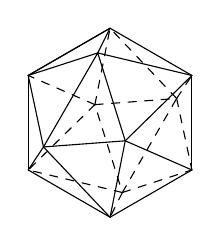
\begin{tikzpicture}[line cap=round,line join=round,scale=0.6]
\foreach \x in {90, 150,..., 450}
{\draw (\x :2)--(\x + 60:2);}
\foreach \x in {30, 90, 150}
{\draw[dashed] (130 :.5)--(\x + 60 :2);}
\foreach \x in {150, 90, 30}
{\draw[dashed] (20 :1.5)--(\x - 60 :2);}
\foreach \x in {150, 210, 270}
{\draw[dashed] (280 :1.5)--(\x + 60 :2);}
\draw[dashed] (130 :.5) -- (20 :1.5) -- (280 :1.5) -- cycle;
\foreach \x in {210, 270, 330}
{\draw (310 :.5)--(\x + 60 :2);}
\foreach \x in {-30, 30, 90}
{\draw (100 :1.5)--(\x + 60 :2);}
\foreach \x in {90, 150, 210}
{\draw (200 :1.5)--(\x + 60 :2);}
\draw (310 :.5) -- (100 :1.5) -- (200 :1.5) -- cycle;
\end{tikzpicture}
\end{center}
Khối tứ diện đều Khối lập phương Bát diện đều Hình 12 mặt đều Hình 20 mặt đều.\\ 
\begin{longtable}[c]{|c|l|l|l|l|>{\centering}p{1cm}|>{\centering}p{1cm}|}
\hline 
\multicolumn{2}{|>{\centering}p{0.3\columnwidth}|}{%
	\begin{minipage}[c]{0.35\textwidth}%
		\begin{center}
			\textbf{Khối đa diện đều}
			\par\end{center}%
\end{minipage} } & \textbf{Số đỉnh} & \textbf{Số cạnh}&\textbf{Số mặt}&\textbf{Loại}&\textbf{Số MPĐX}\tabularnewline
\hline 
\begin{minipage}[c]{0.15\textwidth}%
	\begin{center}
		\textbf{Tứ diện đều}
		\par\end{center}%
\end{minipage}  & %
\begin{minipage}[c]{0.2\textwidth}%
	\begin{center}
		{\begin{tikzpicture}[scale=0.8]
			\tkzDefPoints{0/0/A, 4/0/B, 2/-1/C, 1/3/D}
			\tkzDrawPoints[fill=black](A,B,C,D)
			\tkzDrawSegments[dashed](A,B)
			\tkzDrawSegments(D,A D,B D,C A,C B,C)
			\end{tikzpicture}}
		\par\end{center}%
\end{minipage}  & %
\begin{minipage}[c]{1cm}%
	\begin{center}
		$4$
		\par\end{center}%
\end{minipage}  & %
\begin{minipage}[c]{1cm}%
	\begin{center}
		$6$
		\par\end{center}%
\end{minipage}  & %
\begin{minipage}[c]{1cm}%
	\begin{center}
		$4$
		\par\end{center}%
\end{minipage}  & %
\begin{minipage}[c]{0.2cm}%
	\begin{center}
		\{3;3\}
		\par\end{center}%
\end{minipage} & %
\begin{minipage}[c]{1cm}%
	\begin{center}
		$6$
		\par\end{center}%
\end{minipage}  \tabularnewline
\hline
\begin{minipage}[c]{0.15\textwidth}%
	\begin{center}
		\textbf{Khối lập phương}
		\par\end{center}%
\end{minipage} & %
\begin{minipage}[c]{0.2\textwidth}%
	\begin{center}
		{\begin{tikzpicture}[>=stealth,line join=round,line cap=round,scale=.7]
			\tkzDefPoints{0/0/D,1/2/A,4/2/B,3/0/C,0/3/D'}
			\tkzDefPointBy[translation=from D to D'](A)\tkzGetPoint{A'}
			\tkzDefPointBy[translation=from D to D'](B)\tkzGetPoint{B'}
			\tkzDefPointBy[translation=from D to D'](C)\tkzGetPoint{C'}
			\tkzDrawSegments[](B,C C,D D,D' C,C' B,B' A',B' B',C' C',D' D',A')
			\tkzDrawSegments[dashed](A,B A,D A,A')
			\end{tikzpicture}}
		\par\end{center}%
\end{minipage}  & %
\begin{minipage}[c]{1cm}%
	\begin{center}
		$8$
		\par\end{center}%
\end{minipage}  & %
\begin{minipage}[c]{1cm}%
	\begin{center}
		$12$
		\par\end{center}%
\end{minipage}  & %
\begin{minipage}[c]{1cm}%
	\begin{center}
		$6$
		\par\end{center}%
\end{minipage}  & %
\begin{minipage}[c]{0.2cm}%
	\begin{center}
		\{4;3\}
		\par\end{center}%
\end{minipage} &%
\begin{minipage}[c]{1cm}%
	\begin{center}
		$9$
		\par\end{center}%
\end{minipage}  \tabularnewline
\hline
\begin{minipage}[c]{0.15\textwidth}%
	\begin{center}
		\textbf{Bát diện đều}
		\par\end{center}%
\end{minipage} & %
\begin{minipage}[c]{0.2\textwidth}%
	\begin{center}
		{\begin{tikzpicture}[line cap=round,line join=round,color=cyan,very thick]
			\tkzDefPoints{0/0/O, -.5/.4/A, 1.5/.4/B}
			\coordinate (S) at ($(O)+(0,1.5)$);
			\tkzDefPointBy[symmetry = center O](A) \tkzGetPoint{C}
			\tkzDefPointBy[symmetry = center O](B) \tkzGetPoint{D}
			\tkzDefPointBy[symmetry = center O](S) \tkzGetPoint{S'}
			\tkzDrawSegments[dashed](S,A A,B A,D A,S')
			\tkzDrawPolygon(S,C,D)
			\tkzDrawPolygon(S',B,C)
			\tkzDrawSegments(S,B S',D)
			\end{tikzpicture}}
		\par\end{center}%
\end{minipage}  & %
\begin{minipage}[c]{1cm}%
	\begin{center}
		$6$
		\par\end{center}%
\end{minipage}  & %
\begin{minipage}[c]{1cm}%
	\begin{center}
		$12$
		\par\end{center}%
\end{minipage}  & %
\begin{minipage}[c]{1cm}%
	\begin{center}
		$8$
		\par\end{center}%
\end{minipage}  & %
\begin{minipage}[c]{0.2cm}%
	\begin{center}
		\{3;4\}
		\par\end{center}%
\end{minipage} &%
\begin{minipage}[c]{1cm}%
	\begin{center}
		$9$
		\par\end{center}%
\end{minipage}  \tabularnewline
\hline
\begin{minipage}[c]{0.15\textwidth}%
	\begin{center}
		\textbf{Mười hai mặt đều}
		\par\end{center}%
\end{minipage} & %
\begin{minipage}[c]{0.2\textwidth}%
	\begin{center}
		{\begin{tikzpicture}[scale=0.55,thick,>=stealth',color=black]
			\begin{scope}[rotate=25]
			\draw[black](0,0)coordinate(a1)--++(0:2)coordinate(a2)--++(72:2)coordinate(a3)--++(144:2)coordinate(a4)--++(216:2)coordinate(a5)--(0,0);
			\draw[dashed] (0,2.7)coordinate(b1)--++(0:2)coordinate(b2)--++(-72:2)coordinate(b3)--++(-144:2)coordinate(b4)--++(-216:2)coordinate(b5)--(0,2.7);
			\draw[black] (a4)--++(90:1.2)coordinate(c1)(a1)--++(235:1.2)coordinate(c2)(a2)--++(-52:1.2)coordinate(c3)(a3)--++(18:1.2)coordinate(c4)(a5)--++(165:1.2)coordinate(c5);
			\draw[dashed] (b5)--++(195:1.2)coordinate(c6)(b4)--++(-90:1.2)coordinate(c7)(b3)--++(-17:1.2)coordinate(c8)(b2)--++(56:1.2)coordinate(c9)(b1)--++(126:1.2)coordinate(c);
			\draw[black] (c1)--(c)--(c5)--(c6)--(c2)--(c7)--(c3)--(c8)--(c4)--(c9)--(c1);
			\end{scope}
			\end{tikzpicture}}
		\par\end{center}%
\end{minipage}  & %
\begin{minipage}[c]{1cm}%
	\begin{center}
		$20$
		\par\end{center}%
\end{minipage}  & %
\begin{minipage}[c]{1cm}%
	\begin{center}
		$30$
		\par\end{center}%
\end{minipage}  & %
\begin{minipage}[c]{1cm}%
	\begin{center}
		$12$
		\par\end{center}%
\end{minipage}  & %
\begin{minipage}[c]{0.2cm}%
	\begin{center}
		\{5;3\}
		\par\end{center}%
\end{minipage} &%
\begin{minipage}[c]{1cm}%
	\begin{center}
		$15$
		\par\end{center}%
\end{minipage}  \tabularnewline
\hline
\begin{minipage}[c]{0.15\textwidth}%
	\begin{center}
		\textbf{Hai mươi mặt đều}
		\par\end{center}%
\end{minipage} & %
\begin{minipage}[c]{0.2\textwidth}%
	\begin{center}
		{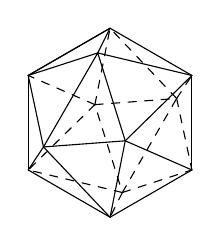
\begin{tikzpicture}[line cap=round,line join=round,scale=0.6]
			\foreach \x in {90, 150,..., 450}
			{\draw (\x :2)--(\x + 60:2);}
			\foreach \x in {30, 90, 150}
			{\draw[dashed] (130 :.5)--(\x + 60 :2);}
			\foreach \x in {150, 90, 30}
			{\draw[dashed] (20 :1.5)--(\x - 60 :2);}
			\foreach \x in {150, 210, 270}
			{\draw[dashed] (280 :1.5)--(\x + 60 :2);}
			\draw[dashed] (130 :.5) -- (20 :1.5) -- (280 :1.5) -- cycle;
			\foreach \x in {210, 270, 330}
			{\draw (310 :.5)--(\x + 60 :2);}
			\foreach \x in {-30, 30, 90}
			{\draw (100 :1.5)--(\x + 60 :2);}
			\foreach \x in {90, 150, 210}
			{\draw (200 :1.5)--(\x + 60 :2);}
			\draw (310 :.5) -- (100 :1.5) -- (200 :1.5) -- cycle;
			\end{tikzpicture}}
		\par\end{center}%
\end{minipage}  & %
\begin{minipage}[c]{1cm}%
	\begin{center}
		$12$
		\par\end{center}%
\end{minipage}  & %
\begin{minipage}[c]{1cm}%
	\begin{center}
		$30$
		\par\end{center}%
\end{minipage}  & %
\begin{minipage}[c]{1cm}%
	\begin{center}
		$20$
		\par\end{center}%
\end{minipage}  & %
\begin{minipage}[c]{0.2cm}%
	\begin{center}
		\{3;5\}
		\par\end{center}%
\end{minipage} &%
\begin{minipage}[c]{1cm}%
	\begin{center}
		$15$
		\par\end{center}%
\end{minipage}  \tabularnewline
\hline 
\end{longtable}
\begin{note}
	Gọi $D$ là tổng số đỉnh, $C$ là tổng số cạnh và $M$ là tổng các mặt của khối đa diện đều loại $\{n;p\}$.
\end{note}
Ta có: \[pD=2C=nM\]
Xét tứ diện đều:\\
$\{3;3\}\to\heva{&n=3, p=3\\&M=4}\xrightarrow{{pD=2C=nM}}C=\dfrac{nM}{2}=6;D=\dfrac{nM}{p}=4$.\\
Xét khối lập phương:\\
 $\{4;3\}\to\heva{&n=4, p=3\\&M=6}\xrightarrow{{pD=2C=nM}}C=\dfrac{nM}{2}=12;D=\dfrac{nM}{p}=8$.\\
Xét bát diện đều:\\
 $\{3;4\}\to\heva{&n=3, p=4\\&M=8}\xrightarrow{pD=2C=nM}C=\dfrac{nM}{2}=12;D=\dfrac{nM}{p}=6$.\\
Xét khối mười hai mặt đều:\\
 $\{5;3\}\to\heva{&n=5, p=3\\&M=12}\xrightarrow{{pD=2C=nM}}C=\dfrac{nM}{2}=30;D=\dfrac{nM}{p}=20$.\\
Xét khối hai mươi mặt đều:\\
 $\{3;5\}\to\heva{&n=3, p=5\\&M=20}\xrightarrow{{pD=2C=nM}}C=\dfrac{nM}{2}=30;D=\dfrac{nM}{p}=12$.\\
Một số kết quả quan trọng về khối đa diện lồi:
\begin{itemize}
	\item Cho một khối tứ diện đều. Khi đó:\\
	Các trọng tâm của các mặt của nó là các đỉnh của một khối tứ diện đều;\\
	Các trung điểm của các cạnh của nó là các đỉnh của một khối bát diện đều (khối tám mặt đều).
	\item Tâm của các mặt của một khối lập phương là các đỉnh của một khối bát diện đều.
	\item Tâm của các mặt của một khối bát diện đều là các đỉnh của một khối lập phương.
	\item Hai đỉnh của một khối bát diện đều được gọi là hai đỉnh đối diện nếu chúng không cùng thuộc một cạnh của khối đó. Đoạn thẳng nối hai đỉnh đối diện gọi là đường chéo của khối bát diện đều. Khi đó:\\
	Ba đường chéo cắt nhau tại trung điểm của mỗi đường.\\
	Ba đường chéo đôi một vuông góc với nhau;\\
	Ba đường chéo bằng nhau.
	\end{itemize}
\subsection{Phân loại và phương pháp giải bài tập}
\begin{dang}{Nhận dạng khối đa diện lồi-Khối đa diện đều}
	Dựa vào định nghĩa và các tính chất của của khối đa diện lồi.\\
	Một khối đa diện được gọi là khối đa diện lồi nếu với bất kì hai điểm $A$ và $B$ nào của nó thì mọi điểm của đoạn $AB$ cũng thuộc khối đó.
\end{dang}
\paragraph{Câu hỏi trắc nghiệm}
\begin{ex}%Câu 1.%[Bùi Đức Thăng]%[2H1Y2-1]
	Cho các hình khối sau:\\ 
	\begin{minipage}{0.27\textwidth}
		\begin{center}
			\begin{tikzpicture}[scale=0.7, font=\footnotesize,
			line join=round, line cap=round, >=stealth]
			\tkzDefPoints{0/0/A, 4/0/D, -1.5/-1.5/B, 0.5/3/A', 3/3/D', -0.5/2/B'}
			\coordinate (C) at ($(D)-(A)+(B)$);
			\coordinate (C') at ($(D')-(A')+(B')$);
			\tkzDrawSegments(A',B' B',C' C',D' D',A' B,B' C,C' D,D' B,C C,D)
			\tkzDrawSegments[dashed](A,A' A,B A,D)
			\node at (1.5,-2){\textbf{Hình 1}};
			\end{tikzpicture}
		\end{center}
	\end{minipage}
	\begin{minipage}{0.13\textwidth}
		\begin{center}
			\begin{tikzpicture}[scale=0.7, font=\footnotesize,
			line join=round, line cap=round, >=stealth]
			\tkzDefPoints{0/0/A, 4/0/D, 1/-1/B, 0/3/x}
			\coordinate (C) at ($(D)-(A)+(B)$);
			\coordinate (A') at ($(A)+(x)$);
			\coordinate (B') at ($(B)+(x)$);
			\coordinate (C') at ($(C)+(x)$);
			\coordinate (D') at ($(D)+(x)$);
			\coordinate (M) at ($(B')!0.6!(C')$);
			\coordinate (N) at ($(M)+(-0.2,0.6)$);
			\coordinate (P) at ($(M)+(0.4,0.6)$);
			\coordinate (M') at ($(M)+(-2,1)$);
			\coordinate (N') at ($(N)+(-2,1)$);
			\coordinate (P') at ($(P)+(-2,1)$);
			\tkzInterLL(P,P')(D',A')\tkzGetPoint{I}
			\tkzDrawSegments(A,B B,C A,A' A',B' B',C' C',D' M,N N,P P,M B,B' C,C' A',M' I,D' M,M' N,N' P,P' M',N' N',P')
			\tkzDrawSegments[dashed](D,A D,D' D,C M',I M',P')
			\node at (2.5,-2){\textbf{Hình 2}};
			\end{tikzpicture}			
		\end{center}
	\end{minipage}
	\begin{minipage}{0.35\textwidth}
		\begin{center}
			
\begin{tikzpicture}[>=stealth,line join=round,line cap=round,scale=0.6, font=\footnotesize]
			\tkzDefPoints{0/0/D,1/2/A,4/2/B,3/0/C,0/3/D'}
			\tkzDefPointBy[translation=from D to D'](A)\tkzGetPoint{A'}
			\tkzDefPointBy[translation=from D to D'](B)\tkzGetPoint{B'}
			\tkzDefPointBy[translation=from D to D'](C)\tkzGetPoint{C'}
			\tkzDrawSegments[](B,C C,D D,D' C,C' B,B' A',B' B',C' C',D' D',A')
			\tkzDrawSegments[dashed](A,B A,D A,A')
			\node at (2.5,-1.5){\textbf{Hình 3}};
			\end{tikzpicture}			
		\end{center}
	\end{minipage}
	\begin{minipage}{0.2\textwidth}
		\begin{center}
			\begin{tikzpicture}[scale=0.6, font=\footnotesize,
			line join=round, line cap=round, >=stealth]
			\tkzDefPoints{0/0/A, 5/0/D, 1/-1/B, 0/3.5/x,1/0.8/y}
			\coordinate (C) at ($(D)-(A)+(B)$);
			\coordinate (A') at ($(A)+(x)$);
			\coordinate (B') at ($(B)+(x)$);
			\coordinate (C') at ($(C)+(x)$);
			\coordinate (D') at ($(D)+(x)$);
			\coordinate (M) at ($(B')+(y)$);
			\coordinate (N) at ($(A')+(y)$);
			\tkzDrawSegments(A,B B,C A',B' B',C' C',D' B',M M,C' A',N N,D' A,A' B,B' C,C' M,N)
			\tkzDrawSegments[dashed](D,A D,C D,D' A',D')
			\node at (3,-2){\textbf{Hình 4}};
			\end{tikzpicture}			
		\end{center}
	\end{minipage}\\
	Mỗi hình trên gồm một số hữu hạn đa giác phẳng (kể cả các điểm trong của nó), hình không phải đa diện lồi là
	\choice
	{Hình 1}
	{\True Hình 2}
	{Hình 3}
	{Hình 4}
	\loigiai{Hình 2.}
\end{ex}
\begin{ex}%Câu 2.%[Bùi Đức Thăng]%[2H1Y2-1]
	Cho các hình khối sau:\\ 
	\begin{minipage}{0.27\textwidth}
		\begin{center}
			\begin{tikzpicture}[scale=0.7, font=\footnotesize,
			line join=round, line cap=round, >=stealth]
			\tkzDefPoints{0/0/A, 4/0/D, -1.5/-1.5/B, 0.5/3/A', 3/3/D', -0.5/2/B'}
			\coordinate (C) at ($(D)-(A)+(B)$);
			\coordinate (C') at ($(D')-(A')+(B')$);
			\tkzDrawSegments(A',B' B',C' C',D' D',A' B,B' C,C' D,D' B,C C,D)
			\tkzDrawSegments[dashed](A,A' A,B A,D)
			\node at (1.5,-2){\textbf{Hình 1}};
			\end{tikzpicture}
		\end{center}
	\end{minipage}
	\begin{minipage}{0.13\textwidth}
		\begin{center}
			\begin{tikzpicture}[scale=0.7, font=\footnotesize,
			line join=round, line cap=round, >=stealth]
			\tkzDefPoints{0/0/A, 4/0/D, 1/-1/B, 0/3/x}
			\coordinate (C) at ($(D)-(A)+(B)$);
			\coordinate (A') at ($(A)+(x)$);
			\coordinate (B') at ($(B)+(x)$);
			\coordinate (C') at ($(C)+(x)$);
			\coordinate (D') at ($(D)+(x)$);
			\coordinate (M) at ($(B')!0.6!(C')$);
			\coordinate (N) at ($(M)+(-0.2,0.6)$);
			\coordinate (P) at ($(M)+(0.4,0.6)$);
			\coordinate (M') at ($(M)+(-2,1)$);
			\coordinate (N') at ($(N)+(-2,1)$);
			\coordinate (P') at ($(P)+(-2,1)$);
			\tkzInterLL(P,P')(D',A')\tkzGetPoint{I}
			\tkzDrawSegments(A,B B,C A,A' A',B' B',C' C',D' M,N N,P P,M B,B' C,C' A',M' I,D' M,M' N,N' P,P' M',N' N',P')
			\tkzDrawSegments[dashed](D,A D,D' D,C M',I M',P')
			\node at (2.5,-2){\textbf{Hình 2}};
			\end{tikzpicture}
		\end{center}
	\end{minipage}
	\begin{minipage}{0.33\textwidth}
		\begin{center}
			\begin{tikzpicture}[scale=0.7, font=\footnotesize,
			line join=round, line cap=round, >=stealth]
			\tkzDefPoints{0/0/A, 3/0/B, 2/3/D, 0/0.8/x, -2/0/y, 0/1/z}
			\coordinate (C) at ($(B)-(A)+(D)$);
			\coordinate (B') at ($(B)+(x)$);
			\coordinate (C') at ($(C)+(x)$);
			\coordinate (A') at ($(B')+(y)$);
			\coordinate (D') at ($(C')-(B')+(A')$);
			\coordinate (N) at ($(A')+(z)$);
			\coordinate (P) at ($(D')+(z)$);
			\coordinate (M) at ($(A)+(x)+(z)$);
			\coordinate (Q) at ($(P)-(N)+(M)$);
			\tkzDrawSegments(A,B B,C A,M M,N N,P P,Q Q,M N,A' A',B' B',C' C',D' D',A' B,B' C,C' D',P)
			\tkzDrawSegments[dashed](A,D D,C D,Q)
			\node at (2.5,-1){\textbf{Hình 3}};
			\end{tikzpicture}
		\end{center}
	\end{minipage}
	\begin{minipage}{0.2\textwidth}
		\begin{center}
			\begin{tikzpicture}[scale=0.6, font=\footnotesize,
			line join=round, line cap=round, >=stealth]
			\tkzDefPoints{0/0/A, 5/0/D, 1/-1/B, 0/3.5/x,1/0.8/y}
			\coordinate (C) at ($(D)-(A)+(B)$);
			\coordinate (A') at ($(A)+(x)$);
			\coordinate (B') at ($(B)+(x)$);
			\coordinate (C') at ($(C)+(x)$);
			\coordinate (D') at ($(D)+(x)$);
			\coordinate (M) at ($(B')+(y)$);
			\coordinate (N) at ($(A')+(y)$);
			\tkzDrawSegments(A,B B,C A',B' B',C' C',D' B',M M,C' A',N N,D' A,A' B,B' C,C' M,N)
			\tkzDrawSegments[dashed](D,A D,C D,D' A',D')
			\node at (2.5,-2){\textbf{Hình 4}};
			\end{tikzpicture}
		\end{center}
	\end{minipage}\\
	Mỗi hình trên gồm một số hữu hạn đa giác phẳng (kể cả các điểm trong của nó), số đa diện lồi là 
	\choice
	{$1$}
	{\True $2$}
	{$3$}
	{$4$}
	\loigiai{
		Hình 1 và hình 4 là khối đa diện lồi.}
\end{ex}
\begin{ex}%Câu 3.%[Bùi Đức Thăng]%[2H1Y2-1]
	Trong các hình dưới đây hình nào không phải đa diện lồi?\\
	\begin{center}
		\begin{minipage}{4cm}
			\begin{tikzpicture}[scale=0.8]
			\tkzDefPoints{0/0/A, 4/0/B, 3/-1/C, 1/3/D}
			\tkzDrawPoints[fill=black](A,B,C,D)
			\tkzDrawSegments[dashed](A,B)
			\tkzDrawSegments(D,A D,B D,C A,C B,C)
			\end{tikzpicture}
			\centering{\textbf{Hình 1}}
		\end{minipage}
		\begin{minipage}{4cm}
			\begin{tikzpicture}[scale=0.8]
			\tkzDefPoints{0/0/A, 4/0/B, 3/-1/C, 0.5/-1/D, 1/3/S}
			\tkzDrawPoints[fill=black](A,B,C,D,S)
			\tkzDrawSegments[dashed](A,B)
			\tkzDrawSegments(S,A S,B S,C S,D A,D C,D B,C)
			\end{tikzpicture}
			\centering{\textbf{Hình 2}}
		\end{minipage}
		\begin{minipage}{4cm}
			\begin{tikzpicture}[scale=0.8]
			\tkzDefPoints{0/0/A, 3/0/B, 2/-1/C, 0/3/A'}
			\tkzDefPointBy[translation=from A to A'](B)\tkzGetPoint{B'}
			\tkzDefPointBy[translation=from A to A'](C)\tkzGetPoint{C'}
			\tkzDrawPoints[fill=black](A,B,C,A',B',C')
			\tkzDrawSegments[dashed](A,B)
			\tkzDrawSegments(A',A B,B' C,C' A,C C,B A',B' B',C' C',A')
			\end{tikzpicture}\\
			\centering{\textbf{Hình 3}}
		\end{minipage}
		\begin{minipage}{4cm}
			\begin{tikzpicture}[scale=0.8]
			\tkzDefPoints{0/0/A, 4/0/B, 3/-1/C, 1/-1/D, 1.5/-0.5/E, 0.3/3/S}
			\tkzDrawPoints[fill=black](A,B,C,D,E,S)
			\tkzInterLL(A,E)(S,D)\tkzGetPoint{I}
			\tkzDrawSegments[dashed](A,B S,E D,E I,E)
			\tkzDrawSegments(S,A S,B S,C S,D B,C C,D A,I)
			\end{tikzpicture}
			\centering{\textbf{Hình 4}}
		\end{minipage}
	\end{center}
	\choice
	{Hình 1}
	{Hình 2}
	{Hình 3}
	{\True Hình 4}
	\loigiai{
		Hình 4 là không phải là khối đa diện lồi.}
\end{ex}
\begin{ex}%Câu 4.%[Bùi Đức Thăng]%[2H1Y2-1]
	Số hình đa diện lồi trong các hình dưới đây là:\\ 
	\begin{center}
		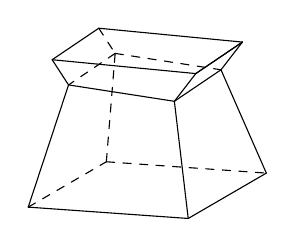
\begin{tikzpicture}[line cap=round,line join=round,>=stealth,x=1.0cm,y=1.0cm,scale=.8]
		\draw [dashed] (0,0)-- (1.24,0.72);
		\draw [dashed] (1.24,0.72)-- (3.78,0.54);
		\draw  (0,0)-- (2.54,-0.18);
		\draw  (2.54,-0.18)-- (3.78,0.54);
		\draw  (0,0)-- (0.64,1.94);
		\draw [dashed] (1.24,0.72)-- (1.38,2.44);
		\draw [dashed] (1.38,2.44)-- (0.64,1.94);
		\draw  (0.64,1.94)-- (2.32,1.68);
		\draw  (2.32,1.68)-- (3.06,2.18);
		\draw  (3.06,2.18)-- (3.78,0.54);
		\draw  (2.32,1.68)-- (2.54,-0.18);
		\draw [dashed] (1.38,2.44)-- (3.06,2.18);
		\draw  (0.64,1.94)-- (0.38,2.34);
		\draw  (2.32,1.68)-- (2.66,2.12);
		\draw  (0.38,2.34)-- (1.12,2.84);
		\draw [dashed] (1.12,2.84)-- (1.38,2.44);
		\draw  (1.12,2.84)-- (3.4,2.62);
		\draw  (3.4,2.62)-- (2.66,2.12);
		\draw  (3.4,2.62)-- (2.66,2.12);
		\draw  (2.66,2.12)-- (0.38,2.34);
		\draw  (3.4,2.62)-- (3.06,2.18);
		\end{tikzpicture} 
		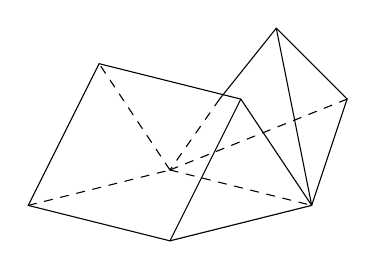
\begin{tikzpicture}[line cap=round,line join=round,>=stealth,x=1.0cm,y=1.0cm,scale=.9]
		\draw [dashed] (0,0)-- (2,0.5);
		\draw [dashed] (2,0.5)-- (4,0);
		\draw  (0,0)-- (2,-0.5);
		\draw  (2,-0.5)-- (4,0);
		\draw [dashed] (2,0.5)-- (1,2);
		\draw  (1,2)-- (0,0);
		\draw  (2,-0.5)-- (3,1.5);
		\draw  (3,1.5)-- (4,0);
		\draw  (3,1.5)-- (1,2);
		\draw  (4,0)-- (3.5,2.5);
		\draw  (3.5,2.5)-- (4.5,1.5);
		\draw  (4.5,1.5)-- (4,0);
		\draw  (3.5,2.5)-- (2.7,1.5);
		\draw [dashed] (2.7,1.5)-- (2.,0.5);
		\draw [dashed] (2,0.5)-- (4.5,1.5);
		\end{tikzpicture} 
		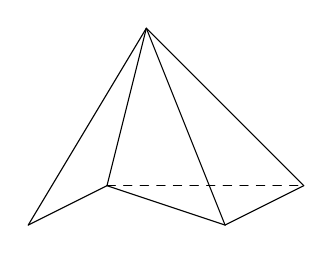
\begin{tikzpicture}[line cap=round,line join=round,>=stealth,x=1.0cm,y=1.0cm,scale=1]
		\draw  (0,0)-- (1,0.5);
		\draw  (1,0.5)-- (2.5,0);
		\draw  (2.5,0)-- (3.5,0.5);
		\draw  (3.5,0.5)-- (1.5,2.5);
		\draw  (1.5,2.5)-- (1,0.5);
		\draw  (1.5,2.5)-- (2.5,0.);
		\draw  (1.5,2.5)-- (0,0);
		\draw [dashed] (1,0.5)-- (3.5,0.5);
		\end{tikzpicture} 
		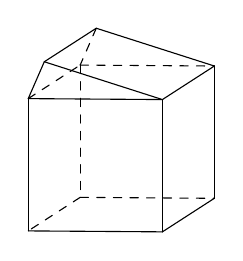
\begin{tikzpicture}[line cap=round,line join=round,>=stealth,x=1.0cm,y=1.0cm,scale=1.2]
		\draw (0,0)-- (0,1.4);
		\draw (0,1.4)-- (1.42,1.39);
		\draw (1.42,1.39)-- (1.42,-0.01);
		\draw (1.42,-0.01)-- (0,0);
		\draw (1.97,0.345)-- (1.42,-0.01);
		\draw (1.97,0.345)-- (1.97,1.745);
		\draw (1.97,1.745)-- (1.42,1.39);
		\draw [dashed] (0.55,1.755)-- (1.97,1.745);
		\draw [dashed] (0.55,1.755)-- (0.55,0.355);
		\draw [dashed] (0.55,0.355)-- (0,0);
		\draw [dashed] (0.55,0.355)-- (1.97,0.345);
		\draw [dashed] (0,1.4)-- (0.55,1.755);
		\draw (0.17,1.79)-- (0.72,2.145);
		\draw [dashed] (0.72,2.145)-- (0.55,1.755);
		\draw (0.17,1.79)-- (1.42,1.39);
		\draw (0.72,2.145)-- (1.97,1.745);
		\draw (0.17,1.79)-- (0,1.4);
		\end{tikzpicture} 	
		\end{center}
	\choice
	{$0$}
	{$2$}
	{$3$}
	{\True $1$}
	\loigiai{.}
\end{ex}
\begin{ex}%Câu 5.%[Bùi Đức Thăng]%[2H1Y2-1]
	Trong các mệnh đề sau, mệnh đề nào \textbf{sai}?
	\choice
	{Hình lập phương là một hình đa diện lồi}
	{Hình hộp là một hình đa diện lồi}
	{Hình tứ diện là một hình đa diện lồi}
	{\True Hình lăng trụ tứ giác là một hình tứ diện lồi}
	\loigiai{
		Theo định nghĩa hình đa diện lồi thì các \lq\lq Hình lập phương là một hình đa diện lồi\rq\rq, \lq\lq Hình hộp là một hình đa diện lồi\rq\rq, \lq\lq Hình tứ diện là một hình đa diện lồi\rq\rq\, đúng.\\
		Hình lăng trụ tứ giác là hình đa diện lồi có $6$ mặt nên \lq\lq Hình lăng trụ tứ giác là một hình tứ diện lồi\rq\rq\, sai.}
\end{ex}
\begin{ex}%Câu 6.%[Bùi Đức Thăng]%[2H1Y2-1]
	Trong các mệnh đề sau, mệnh đề nào \textbf{sai}?
	\choice
	{Hình lập phương là đa diện lồi}
	{Tứ diện là đa diện lồi}
	{Hình hộp là đa diện lồi}
	{\True Hình tạo bởi hai tứ diện đều ghép với nhau là một đa diện lồi}
	\loigiai{.}
\end{ex}
\begin{ex}%Câu 7.%[Bùi Đức Thăng]%[2H1Y2-1]
	Mỗi đỉnh của khối đa diện lồi là đỉnh chung của ít nhất bao nhiêu mặt?
	\choice
	{$2$}
	{$5$}
	{$4$}
	{\True $3$}
	\loigiai{
		Theo lý thuyết.}
\end{ex}
\begin{ex}%Câu 8.%[Bùi Đức Thăng]%[2H1Y2-1]
	Cho các hình khối sau:\\ 
	\begin{minipage}{0.27\textwidth}
		\begin{center}
			\begin{tikzpicture}[scale=0.7, font=\footnotesize,
			line join=round, line cap=round, >=stealth]
			\tkzDefPoints{0/0/A, 4/0/D, -1.5/-1.5/B, 0.5/3/A', 3/3/D', -0.5/2/B'}
			\coordinate (C) at ($(D)-(A)+(B)$);
			\coordinate (C') at ($(D')-(A')+(B')$);
			\tkzDrawSegments(A',B' B',C' C',D' D',A' B,B' C,C' D,D' B,C C,D)
			\tkzDrawSegments[dashed](A,A' A,B A,D)
			\node at (1.5,-2){\textbf{Hình 1}};
			\end{tikzpicture}
		\end{center}
	\end{minipage}
	\begin{minipage}{0.13\textwidth}
		\begin{center}
			\begin{tikzpicture}[scale=0.7, font=\footnotesize,
			line join=round, line cap=round, >=stealth]
			\tkzDefPoints{0/0/A, 4/0/D, 1/-1/B, 0/3/x}
			\coordinate (C) at ($(D)-(A)+(B)$);
			\coordinate (A') at ($(A)+(x)$);
			\coordinate (B') at ($(B)+(x)$);
			\coordinate (C') at ($(C)+(x)$);
			\coordinate (D') at ($(D)+(x)$);
			\coordinate (M) at ($(B')!0.6!(C')$);
			\coordinate (N) at ($(M)+(-0.2,0.6)$);
			\coordinate (P) at ($(M)+(0.4,0.6)$);
			\coordinate (M') at ($(M)+(-2,1)$);
			\coordinate (N') at ($(N)+(-2,1)$);
			\coordinate (P') at ($(P)+(-2,1)$);
			\tkzInterLL(P,P')(D',A')\tkzGetPoint{I}
			\tkzDrawSegments(A,B B,C A,A' A',B' B',C' C',D' M,N N,P P,M B,B' C,C' A',M' I,D' M,M' N,N' P,P' M',N' N',P')
			\tkzDrawSegments[dashed](D,A D,D' D,C M',I M',P')
			\node at (2.5,-2){\textbf{Hình 2}};
			\end{tikzpicture}
		\end{center}
	\end{minipage}
	\begin{minipage}{0.33\textwidth}
		\begin{center}
			\begin{tikzpicture}[scale=0.7, font=\footnotesize,
			line join=round, line cap=round, >=stealth]
			\tkzDefPoints{0/0/A, 3/0/B, 2/3/D, 0/0.8/x, -2/0/y, 0/1/z}
			\coordinate (C) at ($(B)-(A)+(D)$);
			\coordinate (B') at ($(B)+(x)$);
			\coordinate (C') at ($(C)+(x)$);
			\coordinate (A') at ($(B')+(y)$);
			\coordinate (D') at ($(C')-(B')+(A')$);
			\coordinate (N) at ($(A')+(z)$);
			\coordinate (P) at ($(D')+(z)$);
			\coordinate (M) at ($(A)+(x)+(z)$);
			\coordinate (Q) at ($(P)-(N)+(M)$);
			\tkzDrawSegments(A,B B,C A,M M,N N,P P,Q Q,M N,A' A',B' B',C' C',D' D',A' B,B' C,C' D',P)
			\tkzDrawSegments[dashed](A,D D,C D,Q)
			\node at (2.5,-1){\textbf{Hình 3}};
			\end{tikzpicture}
		\end{center}
	\end{minipage}
	\begin{minipage}{0.2\textwidth}
		\begin{center}
			\begin{tikzpicture}[scale=0.6, font=\footnotesize,
			line join=round, line cap=round, >=stealth]
			\tkzDefPoints{0/0/A, 5/0/D, 1/-1/B, 0/3.5/x,1/0.8/y}
			\coordinate (C) at ($(D)-(A)+(B)$);
			\coordinate (A') at ($(A)+(x)$);
			\coordinate (B') at ($(B)+(x)$);
			\coordinate (C') at ($(C)+(x)$);
			\coordinate (D') at ($(D)+(x)$);
			\coordinate (M) at ($(B')+(y)$);
			\coordinate (N) at ($(A')+(y)$);
			\tkzDrawSegments(A,B B,C A',B' B',C' C',D' B',M M,C' A',N N,D' A,A' B,B' C,C' M,N)
			\tkzDrawSegments[dashed](D,A D,C D,D' A',D')
			\node at (2.5,-2){\textbf{Hình 4}};
			\end{tikzpicture}
		\end{center}
	\end{minipage}\\
	Hỏi có bao nhiêu khối đa diện lồi?
	\choice
	{$3$}
	{$4$}
	{$2$}
	{\True $1$}
	\loigiai{
		Ta thấy Hình 1 và Hình 4 là các khối đa diện lồi.}
\end{ex}
\begin{ex}%Câu 9.%[Bùi Đức Thăng]%[2H1Y2-1]
	Khối đa diện đều nào sau đây có mặt không phải là tam giác đều?
	\choice
	{\True Mười hai mặt đều}
	{Hai mươi mặt đều}
	{Tám mặt đều}
	{Tứ diện đều}
	\loigiai	{\text{}\begin{tikzpicture}[scale=0.55,thick,>=stealth',color=black]
		\begin{scope}[rotate=25]
		\draw[black](0,0)coordinate(a1)--++(0:2)coordinate(a2)--++(72:2)coordinate(a3)--++(144:2)coordinate(a4)--++(216:2)coordinate(a5)--(0,0);
		\draw[dashed] (0,2.7)coordinate(b1)--++(0:2)coordinate(b2)--++(-72:2)coordinate(b3)--++(-144:2)coordinate(b4)--++(-216:2)coordinate(b5)--(0,2.7);
		\draw[black] (a4)--++(90:1.2)coordinate(c1)(a1)--++(235:1.2)coordinate(c2)(a2)--++(-52:1.2)coordinate(c3)(a3)--++(18:1.2)coordinate(c4)(a5)--++(165:1.2)coordinate(c5);
		\draw[dashed] (b5)--++(195:1.2)coordinate(c6)(b4)--++(-90:1.2)coordinate(c7)(b3)--++(-17:1.2)coordinate(c8)(b2)--++(56:1.2)coordinate(c9)(b1)--++(126:1.2)coordinate(c);
		\draw[black] (c1)--(c)--(c5)--(c6)--(c2)--(c7)--(c3)--(c8)--(c4)--(c9)--(c1);
		\end{scope}
		\end{tikzpicture}\\
		Khối 12 mặt đều.}
\end{ex}
\begin{ex}%Câu 10.%[Bùi Đức Thăng]%[2H1Y2-1]
	Trong các mệnh đề sau, mệnh đề nào là \textbf{sai}?
	\choice
	{Tứ diện là đa diện lồi}
	{\True Hình tạo bởi hai tứ diện đều ghép với nhau là một đa diện lồi}
	{Hình lập phương là đa diện lồi}
	{Hình hộp là đa diện lồi}
	\loigiai{.}
\end{ex}
\begin{ex}%Câu 11.%[Bùi Đức Thăng]%[2H1Y2-1]
	Cho khối đa diện đều giới hạn bởi hình đa diện $(H)$, khẳng định nào đây \textbf{sai}?
	\choice
	{Các mặt của $(H)$ là những đa diện đều và có cùng số cạnh}
	{\True Mỗi cạnh của một đa giác của $(H)$ là cạnh chung của nhiều hơn hai đa giác}
	{Khối đa diện đều $(H)$ là một khối đa diện lồi}
	{Mỗi đỉnh của $(H)$ là đỉnh chung của cùng một số cạnh}
	\loigiai{.}
\end{ex}
\begin{ex}%Câu 12.%[Bùi Đức Thăng]%[2H1Y2-1]
	Khối lập phương là khối đa diện đều thuộc loại 
	\choice
	{\True $\{4;3\}$}
	{$\{5;3\}$}
	{$\{3;4\}$}
	{$\{3;3\}$}
	\loigiai{
		Mỗi mặt của khối lập phương là tứ giác đều, mỗi đỉnh là giao của 3 mặt.}
\end{ex}
\begin{ex}%Câu 13.%[Bùi Đức Thăng]%[2H1Y2-1]
	Khối bát diện đều là một khối đa diện lồi loại
	\choice
	{$\{5;3\}$}
	{$\{4;3\}$}
	{\True $\{3;4\}$}
	{$\{3;5\}$}
	\loigiai{
		Khối bát diện đều là khối đa diện đều thuộc loại $\{3;4\}$.\\
		Cần nhớ: Khối đa diện đều mà mỗi mặt là đa giác $p$ cạnh và mỗi đỉnh là đỉnh chung của đúng $q$ mặt. Khối đa diện đều như vậy được gọi là khối đa diện đều loại $\{p;q\}$.}
\end{ex}
\begin{ex}%Câu 14.%[Bùi Đức Thăng]%[2H1Y2-1]
	Cho khối đa diện đều loại $\{4; 3\}$, tên gọi của nó là
	\choice
	{Chóp đều}
	{Tứ diện đều}
	{Bát diện đều}
	{\True Lập phương}
	\loigiai{
		Khối đa diện đều loại $\{p; q\}$. Trong đó.\\
		Mỗi mặt của nó là một đa giác đều $p$ cạnh.\\
		Mỗi đỉnh của nó là đỉnh chung của đúng $q$ mặt.\\
		Vậy khối đa diện đều loại $\{4; 3\}$ tên gọi là lập phương.}
\end{ex}
\begin{ex}%Câu 15.%[Bùi Đức Thăng]%[2H1Y2-1]
	Trong các mệnh đề sau,mệnh đề nào \textbf{sai}?
	\choice
	{Hình lập phương là đa diện lồi}
	{Tứ diện là đa diện lồi}
	{Hình hộp là đa diện lồi}
	{\True Hình tạo bởi hai tứ diện đều ghép với nhau là một đa diện lồi}
	\loigiai{.}
\end{ex}
\begin{ex}%Câu 16.%[Bùi Đức Thăng]%[2H1Y2-1]
	\immini{
		Hình đa diện sau có bao nhiêu cạnh?	
	\choice
	{$11$}
	{\True $20$}
	{$12$}
	{$15$}
	}{
		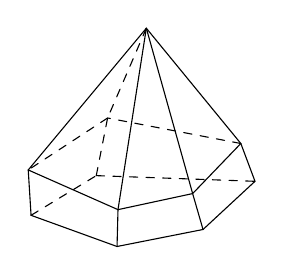
\begin{tikzpicture}[line cap=round,line join=round,>=stealth,x=1.0cm,y=1.0cm,scale=.6]
		\draw (0.24,1.66)-- (2.14,0.82);
		\draw (2.14,0.82)-- (3.72,1.16);
		\draw (3.72,1.16)-- (4.74,2.22);
		\draw [dashed] (4.74,2.22)-- (1.92,2.76);
		\draw [dashed] (1.92,2.76)-- (0.24,1.66);
		\draw (0.24,1.66)-- (2.74,4.66);
		\draw [dashed] (2.74,4.66)-- (1.92,2.76);
		\draw (2.74,4.66)-- (2.14,0.82);
		\draw (3.72,1.16)-- (2.74,4.66);
		\draw  (2.74,4.66)-- (4.74,2.22);
		\draw (0.24,1.66)-- (0.3,0.7);
		\draw [dashed] (0.3,0.7)-- (1.68,1.54);
		\draw [dashed] (1.68,1.54)-- (1.92,2.76);
		\draw [dashed] (1.68,1.54)-- (5.04,1.42);
		\draw  (5.04,1.42)-- (4.74,2.22);
		\draw (5.04,1.42)-- (3.94,0.4);
		\draw (3.94,0.4)-- (3.72,1.16);
		\draw (3.94,0.4)-- (2.12,0.04);
		\draw (2.12,0.04)-- (2.14,0.82);
		\draw (2.12,0.04)-- (0.3,0.7);
		\end{tikzpicture} 
	}
	\loigiai{
		Từ hình vẽ ta thấy khối đa diện này có $20$ cạnh.}
\end{ex}
\begin{ex}%Câu 17.%[Bùi Đức Thăng]%[2H1Y2-1]
	Trong các mệnh đề sau, mệnh đề nào \textbf{sai}?
	\choice
	{Hình lập phương là một hình đa diện lồi}
	{Hình hộp là một hình đa diện lồi}
	{Hình tứ diện là một hình đa diện lồi}
	{\True Hình lăng trụ tứ giác là một hình tứ diện lồi}
	\loigiai{
		Theo định nghĩa hình đa diện lồi thì các phương án \lq\lq Hình lập phương là một hình đa diện lồi\rq\rq, \lq\lq Hình hộp là một hình đa diện lồi\rq\rq\, \lq\lq Hình tứ diện là một hình đa diện lồi\rq\rq\, đúng.\\
		Hình lăng trụ tứ giác là hình đa diện lồi có 6 mặt nên phương án \lq\lq Hình lăng trụ tứ giác là một hình tứ diện lồi\rq\rq\, sai.}
\end{ex}
\begin{ex}%Câu 18.%[Bùi Đức Thăng]%[2H1Y2-1]
	Trong các mệnh đề sau, mệnh đề nào đúng?
	\choice
	{Khối chóp tứ giác đều là khối đa diện đều loại {3;3}}
	{Khối bát diện đều không phải là khối đa diện lồi}
	{Lắp ghép hai khối hộp luôn được một khối đa diện lồi}
	{\True Tồn tại hình đa diện có số đỉnh bằng số mặt}
	\loigiai{
		khối đa diện đều loại {3;3} là khối tứ diện đều. Loại A.\\
		Khối đa diện đều là khối đa diện lồi. Loại B.\\
		Lắp ghép hai khối hộp có mặt không bằng nhau được một khối đa diện không lồi. Loại C.\\
		Hình tứ diện có 4 đỉnh, 4 mặt.}
\end{ex}
\begin{ex}%Câu 19.%[Bùi Đức Thăng]%[2H1Y2-1]
	Khẳng định nào sau đây là khẳng định đúng?
	\choice
	{Tứ diện đều là hình có ba cạnh bên bằng nhau}
	{Tứ diện đều là hình có ba mặt là tam giác cân và một mặt là tam giác đều}
	{\True Tứ diện đều là hình có tất cả sáu cạnh bằng nhau}
	{Tứ diện đều là hình có ba mặt là tam giác vuông cân và một mặt là tam giác đều}
	\loigiai{.}
\end{ex}
\begin{ex}%Câu 20.%[Bùi Đức Thăng]%[2H1Y2-1]
	Khối mười hai mặt đều là khối đa diện loại
	\choice
	{$\{4;3\}$}
	{$\{3;5\}$}
	{$\{3;4\}$}
	{\True $\{5;3\}$}
	\loigiai{
		Khối mười hai mặt đều là khối đa diện loại $\{5;3\}$.}
\end{ex}
\begin{dang}{Đếm số mặt, cạnh của một khối đa diện thông qua hình cho trước}
	Gọi $P$ là tổng số đỉnh, $C$ là tổng số cạnh và $M$ là tổng các mặt của khối đa diện đều loại $\{n;p\}$. Ta có $P=2C=nM$.
\end{dang}
\paragraph{Các ví dụ}
\begin{vd}%Ví dụ 1.%[Bùi Đức Thăng]%[2H1Y2-2]
	Trong không gian chỉ có 5 loại khối đa diện đều như hình vẽ.
	\begin{center}
		\begin{tikzpicture}[scale=0.7]
		\tkzDefPoints{0/0/A, 4/0/B, 2/-1/C, 1/3/D}
		\tkzDrawPoints[fill=black](A,B,C,D)
		\tkzDrawSegments[dashed](A,B)
		\tkzDrawSegments(D,A D,B D,C A,C B,C)
		\end{tikzpicture}
		\quad
		\begin{tikzpicture}[>=stealth,line join=round,line cap=round,scale=.5]
		\tkzDefPoints{0/0/D,1/2/A,4/2/B,3/0/C,0/3/D'}
		\tkzDefPointBy[translation=from D to D'](A)\tkzGetPoint{A'}
		\tkzDefPointBy[translation=from D to D'](B)\tkzGetPoint{B'}
		\tkzDefPointBy[translation=from D to D'](C)\tkzGetPoint{C'}
		\tkzDrawSegments[](B,C C,D D,D' C,C' B,B' A',B' B',C' C',D' D',A')
		\tkzDrawSegments[dashed](A,B A,D A,A')
		\end{tikzpicture}
		\quad
		\begin{tikzpicture}[line cap=round,line join=round,color=cyan,scale=1]
		\tkzDefPoints{0/0/O, -.5/.4/A, 1.5/.4/B}
		\coordinate (S) at ($(O)+(0,1.5)$);
		\tkzDefPointBy[symmetry = center O](A) \tkzGetPoint{C}
		\tkzDefPointBy[symmetry = center O](B) \tkzGetPoint{D}
		\tkzDefPointBy[symmetry = center O](S) \tkzGetPoint{S'}
		\tkzDrawSegments[dashed](S,A A,B A,D A,S')
		\tkzDrawPolygon(S,C,D)
		\tkzDrawPolygon(S',B,C)
		\tkzDrawSegments(S,B S',D)
		\end{tikzpicture}
		\quad
		\begin{tikzpicture}[scale=0.50,thick,>=stealth',color=black]
		\begin{scope}[rotate=25]
		\draw[black](0,0)coordinate(a1)--++(0:2)coordinate(a2)--++(72:2)coordinate(a3)--++(144:2)coordinate(a4)--++(216:2)coordinate(a5)--(0,0);
		\draw[dashed] (0,2.7)coordinate(b1)--++(0:2)coordinate(b2)--++(-72:2)coordinate(b3)--++(-144:2)coordinate(b4)--++(-216:2)coordinate(b5)--(0,2.7);
		\draw[black] (a4)--++(90:1.2)coordinate(c1)(a1)--++(235:1.2)coordinate(c2)(a2)--++(-52:1.2)coordinate(c3)(a3)--++(18:1.2)coordinate(c4)(a5)--++(165:1.2)coordinate(c5);
		\draw[dashed] (b5)--++(195:1.2)coordinate(c6)(b4)--++(-90:1.2)coordinate(c7)(b3)--++(-17:1.2)coordinate(c8)(b2)--++(56:1.2)coordinate(c9)(b1)--++(126:1.2)coordinate(c);
		\draw[black] (c1)--(c)--(c5)--(c6)--(c2)--(c7)--(c3)--(c8)--(c4)--(c9)--(c1);
		\end{scope}
		\end{tikzpicture}
		\quad
		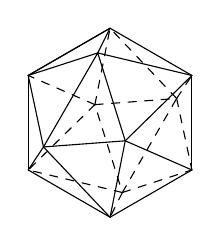
\begin{tikzpicture}[line cap=round,line join=round,scale=0.6]
		\foreach \x in {90, 150,..., 450}
		{\draw (\x :2)--(\x + 60:2);}
		\foreach \x in {30, 90, 150}
		{\draw[dashed] (130 :.5)--(\x + 60 :2);}
		\foreach \x in {150, 90, 30}
		{\draw[dashed] (20 :1.5)--(\x - 60 :2);}
		\foreach \x in {150, 210, 270}
		{\draw[dashed] (280 :1.5)--(\x + 60 :2);}
		\draw[dashed] (130 :.5) -- (20 :1.5) -- (280 :1.5) -- cycle;
		\foreach \x in {210, 270, 330}
		{\draw (310 :.5)--(\x + 60 :2);}
		\foreach \x in {-30, 30, 90}
		{\draw (100 :1.5)--(\x + 60 :2);}
		\foreach \x in {90, 150, 210}
		{\draw (200 :1.5)--(\x + 60 :2);}
		\draw (310 :.5) -- (100 :1.5) -- (200 :1.5) -- cycle;
		\end{tikzpicture}
	\end{center}
	Hãy sáp xêp khối đa diện đều theo thứ tự tăng dần của số đỉnh.
	\loigiai{
		\begin{longtable}[c]{|c|l|>{\centering}p{0.15\textwidth}|>{\centering}p{2cm}|}
			\hline 
			\multicolumn{2}{|>{\centering}p{0.3\columnwidth}|}{%
				\begin{minipage}[c]{0.6\textwidth}%
					\begin{center}
						\textbf{Khối đa diện đều}
						\par\end{center}%
			\end{minipage} } & \textbf{Số đỉnh} & \textbf{Lo\d{a}i}\tabularnewline
			\hline 
			\begin{minipage}[c]{0.3\textwidth}%
				\begin{center}
					\textbf{Tứ diện đều}
					\par\end{center}%
			\end{minipage}  & %
			\begin{minipage}[c]{0.3\textwidth}%
				\begin{center}
					{\begin{tikzpicture}[scale=0.8]
						\tkzDefPoints{0/0/A, 4/0/B, 2/-1/C, 1/3/D}
						\tkzDrawPoints[fill=black](A,B,C,D)
						\tkzDrawSegments[dashed](A,B)
						\tkzDrawSegments(D,A D,B D,C A,C B,C)
						\end{tikzpicture}}
					\par\end{center}%
			\end{minipage}  & %
			\begin{minipage}[c]{2cm}%
				\begin{center}
					$4$
					\par\end{center}%
			\end{minipage}  & %
			\begin{minipage}[c]{2cm}%
				\begin{center}
					\{3;3\}
					\par\end{center}%
			\end{minipage}\tabularnewline
			\hline 
			\begin{minipage}[c]{0.3\textwidth}%
				\begin{center}
					\textbf{Khối lập phương}
					\par\end{center}%
			\end{minipage} & %
			\begin{minipage}[c]{0.3\textwidth}%
				\begin{center}
					{\begin{tikzpicture}[>=stealth,line join=round,line cap=round,scale=.7]
						\tkzDefPoints{0/0/D,1/2/A,4/2/B,3/0/C,0/3/D'}
						\tkzDefPointBy[translation=from D to D'](A)\tkzGetPoint{A'}
						\tkzDefPointBy[translation=from D to D'](B)\tkzGetPoint{B'}
						\tkzDefPointBy[translation=from D to D'](C)\tkzGetPoint{C'}
						\tkzDrawSegments[](B,C C,D D,D' C,C' B,B' A',B' B',C' C',D' D',A')
						\tkzDrawSegments[dashed](A,B A,D A,A')
						\end{tikzpicture}}
					\par\end{center}%
			\end{minipage}  & %
			\begin{minipage}[c]{2cm}%
				\begin{center}
					$8$
					\par\end{center}%
			\end{minipage}  & %
			\begin{minipage}[c]{2cm}%
				\begin{center}
					\{4;3\}
					\par\end{center}%
			\end{minipage}\tabularnewline
			\hline 
			\begin{minipage}[c]{0.3\textwidth}%
				\begin{center}
					\textbf{Bát diện đều}
					\par\end{center}%
			\end{minipage} & %
			\begin{minipage}[c]{0.3\textwidth}%
				\begin{center}
					{\begin{tikzpicture}[line cap=round,line join=round,color=cyan,very thick]
						\tkzDefPoints{0/0/O, -.5/.4/A, 1.5/.4/B}
						\coordinate (S) at ($(O)+(0,1.5)$);
						\tkzDefPointBy[symmetry = center O](A) \tkzGetPoint{C}
						\tkzDefPointBy[symmetry = center O](B) \tkzGetPoint{D}
						\tkzDefPointBy[symmetry = center O](S) \tkzGetPoint{S'}
						\tkzDrawSegments[dashed](S,A A,B A,D A,S')
						\tkzDrawPolygon(S,C,D)
						\tkzDrawPolygon(S',B,C)
						\tkzDrawSegments(S,B S',D)
						\end{tikzpicture}}
					\par\end{center}%
			\end{minipage}  & %
			\begin{minipage}[c]{2cm}%
				\begin{center}
					$6$
					\par\end{center}%
			\end{minipage}  & %
			\begin{minipage}[c]{2cm}%
				\begin{center}
					\{3;4\}
					\par\end{center}%
			\end{minipage} \tabularnewline
			\hline 
			\begin{minipage}[c]{0.3\textwidth}%
				\begin{center}
					\textbf{Mười hai mặt đều}
					\par\end{center}%
			\end{minipage} & %
			\begin{minipage}[c]{0.3\textwidth}%
				\begin{center}
					{\begin{tikzpicture}[scale=0.55,thick,>=stealth',color=black]
						\begin{scope}[rotate=25]
						\draw[black](0,0)coordinate(a1)--++(0:2)coordinate(a2)--++(72:2)coordinate(a3)--++(144:2)coordinate(a4)--++(216:2)coordinate(a5)--(0,0);
						\draw[dashed] (0,2.7)coordinate(b1)--++(0:2)coordinate(b2)--++(-72:2)coordinate(b3)--++(-144:2)coordinate(b4)--++(-216:2)coordinate(b5)--(0,2.7);
						\draw[black] (a4)--++(90:1.2)coordinate(c1)(a1)--++(235:1.2)coordinate(c2)(a2)--++(-52:1.2)coordinate(c3)(a3)--++(18:1.2)coordinate(c4)(a5)--++(165:1.2)coordinate(c5);
						\draw[dashed] (b5)--++(195:1.2)coordinate(c6)(b4)--++(-90:1.2)coordinate(c7)(b3)--++(-17:1.2)coordinate(c8)(b2)--++(56:1.2)coordinate(c9)(b1)--++(126:1.2)coordinate(c);
						\draw[black] (c1)--(c)--(c5)--(c6)--(c2)--(c7)--(c3)--(c8)--(c4)--(c9)--(c1);
						\end{scope}
						\end{tikzpicture}}
					\par\end{center}%
			\end{minipage}  & %
			\begin{minipage}[c]{2cm}%
				\begin{center}
					$20$
					\par\end{center}%
			\end{minipage}  & %
			\begin{minipage}[c]{2cm}%
				\begin{center}
					\{5;3\}
					\par\end{center}%
			\end{minipage}\tabularnewline
			\hline 
			\begin{minipage}[c]{0.3\textwidth}%
				\begin{center}
					\textbf{Hai mươi mặt đều}
					\par\end{center}%
			\end{minipage} & %
			\begin{minipage}[c]{0.3\textwidth}%
				\begin{center}
					{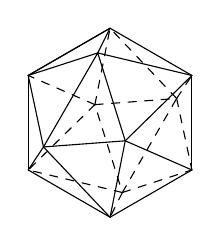
\begin{tikzpicture}[line cap=round,line join=round,scale=0.6]
						\foreach \x in {90, 150,..., 450}
						{\draw (\x :2)--(\x + 60:2);}
						\foreach \x in {30, 90, 150}
						{\draw[dashed] (130 :.5)--(\x + 60 :2);}
						\foreach \x in {150, 90, 30}
						{\draw[dashed] (20 :1.5)--(\x - 60 :2);}
						\foreach \x in {150, 210, 270}
						{\draw[dashed] (280 :1.5)--(\x + 60 :2);}
						\draw[dashed] (130 :.5) -- (20 :1.5) -- (280 :1.5) -- cycle;
						\foreach \x in {210, 270, 330}
						{\draw (310 :.5)--(\x + 60 :2);}
						\foreach \x in {-30, 30, 90}
						{\draw (100 :1.5)--(\x + 60 :2);}
						\foreach \x in {90, 150, 210}
						{\draw (200 :1.5)--(\x + 60 :2);}
						\draw (310 :.5) -- (100 :1.5) -- (200 :1.5) -- cycle;
						\end{tikzpicture}}
					\par\end{center}%
			\end{minipage}  & %
			\begin{minipage}[c]{2cm}%
				\begin{center}
					$12$
					\par\end{center}%
			\end{minipage}  & %
			\begin{minipage}[c]{2cm}%
				\begin{center}
					\{3;5\}
					\par\end{center}%
			\end{minipage}\tabularnewline
			\hline 
		\end{longtable}		
		Vậy khối đa diện đều được sắp xếp theo thứ tự tăng dần của số đỉnh là\\
		$\{3; 3\}$, $\{3; 4\}$, $\{4; 3\}$, $\{3; 5\}$, $\{5; 3\}$.}
\end{vd}
\begin{vd}%Ví dụ 2.%[Bùi Đức Thăng]%[2H1Y2-2]
	\immini{
		Gọi số đỉnh, số cạnh, số mặt của hình đa diện trong hình vẽ bên lần lượt là $a,b,c$. Hỏi $T=a+b-c$ bằng bao nhiêu?	
	}{
		\begin{tikzpicture}[scale=0.55,thick,>=stealth',color=black]
		\begin{scope}[rotate=25]
		\draw[black](0,0)coordinate(a1)--++(0:2)coordinate(a2)--++(72:2)coordinate(a3)--++(144:2)coordinate(a4)--++(216:2)coordinate(a5)--(0,0);
		\draw[dashed] (0,2.7)coordinate(b1)--++(0:2)coordinate(b2)--++(-72:2)coordinate(b3)--++(-144:2)coordinate(b4)--++(-216:2)coordinate(b5)--(0,2.7);
		\draw[black] (a4)--++(90:1.2)coordinate(c1)(a1)--++(235:1.2)coordinate(c2)(a2)--++(-52:1.2)coordinate(c3)(a3)--++(18:1.2)coordinate(c4)(a5)--++(165:1.2)coordinate(c5);
		\draw[dashed] (b5)--++(195:1.2)coordinate(c6)(b4)--++(-90:1.2)coordinate(c7)(b3)--++(-17:1.2)coordinate(c8)(b2)--++(56:1.2)coordinate(c9)(b1)--++(126:1.2)coordinate(c);
		\draw[black] (c1)--(c)--(c5)--(c6)--(c2)--(c7)--(c3)--(c8)--(c4)--(c9)--(c1);
		\end{scope}
		\end{tikzpicture}
	}
	\loigiai{
		Đây là đa diện có $12$ mặt đều. Đây là hình loại $\{5;3\}$. Ta có công thức liên hệ giữa số cạnh, số đỉnh và số mặt của đa diện 12 mặt đều là $3a=2b=5c=5\times 12=60$ \\
		$ \Rightarrow a=20 $, $b=30$. Vậy $T=a+b-c=20+30-12=38$.}
\end{vd}
\begin{vd}%Ví dụ 3.%[Bùi Đức Thăng]%[2H1Y2-2]
	Gọi $x, y, z$ lần lượt là số đỉnh, số cạnh và số mặt của một khối đa diện đều loại $\{3; 4\}$. Tổng $T=x+y+2z$ bằng\\
	Khối đa diện đều loại $\{3; 4\}$ là khối bát diện đều, có $6$ đỉnh, $12$ cạnh và $8$ mặt.\\
	Vậy $T=x+y+2z =6+12+2\cdot 8=34$.
\end{vd}
\paragraph{Câu hỏi trắc nghiệm.}
\begin{ex}%Câu 21.%[Bùi Đức Thăng]%[2H1Y2-2]
	Trong không gian chỉ có 5 loại khối đa diện đều như hình vẽ. \\
\begin{center}
	\begin{tikzpicture}[scale=0.8]
	\tkzDefPoints{0/0/A, 4/0/B, 2/-1/C, 1/3/D}
	\tkzDrawPoints[fill=black](A,B,C,D)
	\tkzDrawSegments[dashed](A,B)
	\tkzDrawSegments(D,A D,B D,C A,C B,C)
	\end{tikzpicture}
	\qquad
	\begin{tikzpicture}[>=stealth,line join=round,line cap=round,scale=.7]
	\tkzDefPoints{0/0/D,1/2/A,4/2/B,3/0/C,0/3/D'}
	\tkzDefPointBy[translation=from D to D'](A)\tkzGetPoint{A'}
	\tkzDefPointBy[translation=from D to D'](B)\tkzGetPoint{B'}
	\tkzDefPointBy[translation=from D to D'](C)\tkzGetPoint{C'}
	\tkzDrawSegments[](B,C C,D D,D' C,C' B,B' A',B' B',C' C',D' D',A')
	\tkzDrawSegments[dashed](A,B A,D A,A')
	\end{tikzpicture}
	\qquad
	\begin{tikzpicture}[line cap=round,line join=round,color=cyan,very thick]
	\tkzDefPoints{0/0/O, -.5/.4/A, 1.5/.4/B}
	\coordinate (S) at ($(O)+(0,1.5)$);
	\tkzDefPointBy[symmetry = center O](A) \tkzGetPoint{C}
	\tkzDefPointBy[symmetry = center O](B) \tkzGetPoint{D}
	\tkzDefPointBy[symmetry = center O](S) \tkzGetPoint{S'}
	\tkzDrawSegments[dashed](S,A A,B A,D A,S')
	\tkzDrawPolygon(S,C,D)
	\tkzDrawPolygon(S',B,C)
	\tkzDrawSegments(S,B S',D)
	\end{tikzpicture}
	\qquad
	\begin{tikzpicture}[scale=0.55,thick,>=stealth',color=black]
	\begin{scope}[rotate=25]
	\draw[black](0,0)coordinate(a1)--++(0:2)coordinate(a2)--++(72:2)coordinate(a3)--++(144:2)coordinate(a4)--++(216:2)coordinate(a5)--(0,0);
	\draw[dashed] (0,2.7)coordinate(b1)--++(0:2)coordinate(b2)--++(-72:2)coordinate(b3)--++(-144:2)coordinate(b4)--++(-216:2)coordinate(b5)--(0,2.7);
	\draw[black] (a4)--++(90:1.2)coordinate(c1)(a1)--++(235:1.2)coordinate(c2)(a2)--++(-52:1.2)coordinate(c3)(a3)--++(18:1.2)coordinate(c4)(a5)--++(165:1.2)coordinate(c5);
	\draw[dashed] (b5)--++(195:1.2)coordinate(c6)(b4)--++(-90:1.2)coordinate(c7)(b3)--++(-17:1.2)coordinate(c8)(b2)--++(56:1.2)coordinate(c9)(b1)--++(126:1.2)coordinate(c);
	\draw[black] (c1)--(c)--(c5)--(c6)--(c2)--(c7)--(c3)--(c8)--(c4)--(c9)--(c1);
	\end{scope}
	\end{tikzpicture}
	\qquad
	\begin{tikzpicture}[line cap=round,line join=round,scale=0.6]
	\foreach \x in {90, 150,..., 450}
	{\draw (\x :2)--(\x + 60:2);}
	\foreach \x in {30, 90, 150}
	{\draw[dashed] (130 :.5)--(\x + 60 :2);}
	\foreach \x in {150, 90, 30}
	{\draw[dashed] (20 :1.5)--(\x - 60 :2);}
	\foreach \x in {150, 210, 270}
	{\draw[dashed] (280 :1.5)--(\x + 60 :2);}
	\draw[dashed] (130 :.5) -- (20 :1.5) -- (280 :1.5) -- cycle;
	\foreach \x in {210, 270, 330}
	{\draw (310 :.5)--(\x + 60 :2);}
	\foreach \x in {-30, 30, 90}
	{\draw (100 :1.5)--(\x + 60 :2);}
	\foreach \x in {90, 150, 210}
	{\draw (200 :1.5)--(\x + 60 :2);}
	\draw (310 :.5) -- (100 :1.5) -- (200 :1.5) -- cycle;
	\end{tikzpicture}
\end{center}
	Mệnh đề nào sau đây đúng?
	\choice
	{Mọi khối đa diện đều có số mặt là những số chia hết cho 4}
	{\True Khối lập phương và khối bát diện đều có cùng số cạnh}
	{Khối tứ diện đều và khối bát diện đều có 1 tâm đối xứng}
	{Khối mười hai mặt đều và khối hai mươi mặt đều có cùng số đỉnh}
	\loigiai{
		Ta có: A sai vì hình bát diện đều không thỏa mãn.\\
		C sai vì tứ diện đều không có tâm đối xứng.\\
		D sai vì khối hai mươi mặt đều có $12$ đỉnh, khối mười hai mặt đều có $20$ đỉnh.\\
		Vậy chỉ có B đúng. Khối lập phương và khối bát diện đều có $12$ cạnh.}
\end{ex}
\begin{ex}%Câu 22.%[Bùi Đức Thăng]%[2H1Y2-2]
	Khối đa diện đều loại $\{4;3\}$ có bao nhiêu đỉnh?
	\choice
	{\True $8$}
	{$6$}
	{$10$}
	{$4$}
	\loigiai{
		Khối đa diện đều loại $\{4;3\}$ là khối lập phương, vậy có 8 đỉnh.}
\end{ex}
\begin{ex}%Câu 23.%[Bùi Đức Thăng]%[2H1Y2-2]
	Tổng số mặt, số cạnh và số đỉnh của hình lập phương là
	\choice
	{\True $26$}
	{$24$}
	{$30$}
	{$32$}
	\loigiai{
		Hình lập phương có $6$ mặt, $12$ cạnh và $8$ đỉnh $\Rightarrow$ tổng số mặt, số cạnh và số đỉnh là $26$.}
\end{ex}
\begin{ex}%Câu 24.%[Bùi Đức Thăng]%[2H1Y2-2]
	Số nào trong các số sau đây \textbf{không} phải là số mặt của một khối đa diện đều nào đó 
	\choice
	{$12$}
	{$20$}
	{$6$}
	{\True $30$}
	\loigiai{.}
\end{ex}
\begin{ex}%Câu 25.%[Bùi Đức Thăng]%[2H1Y2-2]
	Phát biểu nào sau đây là đúng?
	\choice
	{Hình hai mươi mặt đều có 20 đỉnh, 30 cạnh, 12 mặt}
	{Hình hai mươi mặt đều có 30 đỉnh, 12 cạnh, 20 mặt}
	{Hình hai mươi mặt đều có 30 đỉnh, 20 cạnh, 12 mặt}
	{\True Hình hai mươi mặt đều có 12 đỉnh, 30 cạnh, 20 mặt}
	\loigiai{.}
\end{ex}
\begin{ex}%Câu 26.%[Bùi Đức Thăng]%[2H1Y2-2]
	Khẳng định nào sau đây là đúng?
	\choice
	{Hình tứ diện đều có $6$ đỉnh, $6$ cạnh, $4$ mặt}
	{Hình tứ diện đều có $4$ đỉnh, $4$ cạnh, $4$ mặt}
	{Hình tứ diện đều có $6$ đỉnh, $4$ cạnh, $4$ mặt}
	{\True Hình tứ diện đều có $4$ đỉnh, $6$ cạnh, $4$ mặt}
	\loigiai{.}
\end{ex}
\begin{ex}%Câu 27.%[Bùi Đức Thăng]%[2H1Y2-2]
	Số đỉnh của một hình bát diện đều là bao nhiêu?
	\choice
	{$10$}
	{$8$}
	{\True $6$}
	{$12$}
	\loigiai{
		Hình bát diện đều có 6 đỉnh.}
\end{ex}
\begin{ex}%Câu 28.%[Bùi Đức Thăng]%[2H1Y2-2]
	Số cạnh của một hình bát diện đều là 
	\choice
	{Tám}
	{Mười sáu}
	{\True Mười hai}
	{Mười}
	\loigiai{.}
\end{ex}
\begin{ex}%Câu 29.%[Bùi Đức Thăng]%[2H1Y2-2]
	Gọi $d$ là số đỉnh và $m$ là số mặt của khối đa diện đều loại $\{3;4\}$. Mệnh đề nào dưới đây đúng. 
	\choice
	{\True $d=6$, $m=8$}
	{$d=8$, $m=6$}
	{$d=4$, $m=6$}
	{$d=6$, $m=4$}
	\loigiai{
		Khối bát diện đều có $6$ đỉnh và $8$ mặt.}
\end{ex}
\begin{ex}%Câu 30.%[Bùi Đức Thăng]%[2H1Y2-2]
	Kí hiệu $M$ là số mặt, là số đỉnh và $C$ là số cạnh của một hình bát diện đều. Khi đó bộ tương ứng với bộ số nào?
	\choice
	{}
	{}
	{\True}
	{}
	\loigiai{
		Hình bát diện đều có 8 mặt, mỗi mặt là tam giác đều, có 6 đỉnh và 12 cạnh.}
\end{ex}
\begin{ex}%Câu 31.%[Bùi Đức Thăng]%[2H1Y2-2]
	Hình mười hai mặt đều có bao nhiêu cạnh?
	\choice
	{$12$}
	{$18$}
	{\True $30$}
	{$20$}
	\loigiai{.}
\end{ex}
\begin{ex}%Câu 32.%[Bùi Đức Thăng]%[2H1Y2-2]
	Hình đa diện đều có tất cả các mặt là ngũ giác có bao nhiêu cạnh?
	\choice
	{$60$}
	{$20$}
	{$12$}
	{\True $30$}
	\loigiai\\{
	\begin{tikzpicture}[scale=0.55,thick,>=stealth',color=black]
	\begin{scope}[rotate=25]
	\draw[black](0,0)coordinate(a1)--++(0:2)coordinate(a2)--++(72:2)coordinate(a3)--++(144:2)coordinate(a4)--++(216:2)coordinate(a5)--(0,0);
	\draw[dashed] (0,2.7)coordinate(b1)--++(0:2)coordinate(b2)--++(-72:2)coordinate(b3)--++(-144:2)coordinate(b4)--++(-216:2)coordinate(b5)--(0,2.7);
	\draw[black] (a4)--++(90:1.2)coordinate(c1)(a1)--++(235:1.2)coordinate(c2)(a2)--++(-52:1.2)coordinate(c3)(a3)--++(18:1.2)coordinate(c4)(a5)--++(165:1.2)coordinate(c5);
	\draw[dashed] (b5)--++(195:1.2)coordinate(c6)(b4)--++(-90:1.2)coordinate(c7)(b3)--++(-17:1.2)coordinate(c8)(b2)--++(56:1.2)coordinate(c9)(b1)--++(126:1.2)coordinate(c);
	\draw[black] (c1)--(c)--(c5)--(c6)--(c2)--(c7)--(c3)--(c8)--(c4)--(c9)--(c1);
	\end{scope}
	\end{tikzpicture}\\
		Hình đa diện đều duy nhất có tất cả các mặt là ngũ giác chính là hình mười hai mặt đều. Hình này có $30$ cạnh, 20 đỉnh và 12 mặt.}
\end{ex}
\begin{ex}%Câu 33.%[Bùi Đức Thăng]%[2H1Y2-2]
	Số đỉnh và số cạnh của hình hai mươi mặt là tam giác đều là
	\choice
	{\True $12$ đỉnh và $30$ cạnh}
	{$24$ đỉnh và $30$ cạnh}
	{$24$ đỉnh và $24$ cạnh}
	{$12$ đỉnh và $24$ cạnh}
	\loigiai{
		Hình đa diện đều duy nhất có tất cả các mặt là ngũ giác chính là hình mười hai mặt đều. Hình này có $30$ cạnh, 20 đỉnh và 12 mặt.}
\end{ex}
\begin{ex}%Câu 34.%[Bùi Đức Thăng]%[2H1Y2-2]
	Khối đa diện đều nào sau có số đỉnh nhiều nhất?
	\choice
	{Khối nhị thập diện đều ($20$ mặt đều)}
	{Khối tứ diện đều}
	{Khối bát diện đều ($8$ mặt đều)}
	{\True Khối thập nhị diện đều ($12$ mặt đều)}
	\loigiai{.}
\end{ex}
\begin{ex}%Câu 35.%[Bùi Đức Thăng]%[2H1Y2-2]
	Cho khối lập phương. Khẳng định nào sau đây đúng?
	\choice
	{Số mặt của khối lập phương là $4$}
	{\True Khối lập phương là khối đa diện loại $\{4;3\}$.}
	{Số cạnh của khối lập phương là $8$}
	{Khối lập phương là khối đa diện loại $\{3;4\}$}
	\loigiai{
		Khối lập phương có mỗi mặt là một đa giác đều 4 cạnh.\\
		Khối lập phương có mỗi điểm là đỉnh chung của đúng 3 mặt.\\
		Vậy khối lập phương là khối đa diện loại $\{4;3\}$.}
\end{ex}
\begin{ex}%Câu 36.%[Bùi Đức Thăng]%[2H1Y2-2]
	Một khối đa diện lồi với các mặt là tam giác thì
	\choice
	{\True $3M=2C$}
	{$3M>2C$}
	{$3M<2C$}
	{Đáp số khác}
	\loigiai{
		Đa diện lồi có công thức: $pM=qD=2C$. Đa diện lồi có các mặt là tam giác thì $3M=2C$.}
\end{ex}

\begin{ex}%[Phạm Thế Sinh]%[2H1Y1-2]%Câu 36.
	Một khối đa diện lồi với các mặt là tam giác thì
	\choice
	{\True $3M=2C$}
	{$3M>2C$}
	{$3M<2C$}
	{Đáp số khác}
	\loigiai{
		Đa diện lồi có công thức: $pM=qD=2C$. Đa diện lồi có các mặt là tam giác thì $3M=2C$.}
\end{ex}
\begin{ex}%[Phạm Thế Sinh]%[2H1Y1-2]%Câu 37.
	Biết rằng khối đa diện mà mỗi mặt đều là hình ngũ giác. Gọi $C$ là số cạnh của khối đa diện đó, lúc đó ta có
	\choice
	{$C$ là số chia hết cho $3$}
	{$C$ là số chẵn}
	{$C$ là số lẻ}
	{\True $C$ là số chia hết cho $5$}
	\loigiai{
		Gọi $ M $ là số mặt của khối đa diện. Do mỗi mặt của khối đa diện là hình ngũ giác và mỗi cạnh là cạnh chung của đúng $2$ mặt nên ta có $2C=5M$, suy ra $C$ là số chia hết cho $5$.}
\end{ex}
\begin{ex}%[Phạm Thế Sinh]%[2H1Y2-2]%Câu 38.
	Trong tất cả các hình đa diện đều, hình nào có số mặt nhiều nhất?
	\choice
	{\True Hình nhị thập diện đều}
	{Hình thập nhị diện đều}
	{Hình bát diện đều}
	{Hình lập phương}
	\loigiai{
		\begin{itemize}
			\item Hình nhị thập diện đều $20$ mặt.
			\item Hình thập nhị diện đều $12$ mặt.
			\item Hình bát diện đều $8$ mặt.
			\item Hình lập phương $6$ mặt.
	\end{itemize}}	
\end{ex}
\begin{ex}%[Phạm Thế Sinh]%[2H1Y2-2]%Câu 39.
	Khối lập phương là khối đa diện đều loại: 
	\choice
	{$\{5;3\}$}
	{$\{3;4\}$}
	{\True $\{4;3\}$}
	{$\{3;5\}$}
	\loigiai{
		Khối lập phương là khối đa diện đều loại $\{4;3\}$.}
\end{ex}		
\begin{ex}%[Phạm Thế Sinh]%[2H1Y2-2]%Câu 40.
	Khối đa diện đều loại $\{p;q\}$ là khối đa diện có đặc điểm: 
	\choice
	{\True Mỗi mặt là đa giác đều $p$ cạnh và mỗi đỉnh là đỉnh chung của đúng $q$ mặt}
	{Có $p$ mặt là đa giác đều và mỗi đỉnh là đỉnh chung của đúng $q$ cạnh}
	{Có $p$ mặt là đa giác đều và mỗi mặt có $q$ cạnh}
	{Có $q$ mặt là đa giác đều và mỗi mặt có $p$ cạnh}
	\loigiai{
		Một khối đa diện lồi được gọi là \textit{khối đa diện đều} loại $\{p;q\}$ nếu:
		\begin{enumerate}
			\item Mỗi mặt của nó là một đa giác đều $p$ cạnh.
			\item Mỗi đỉnh của nó là đỉnh chung của đúng $q$ mặt.
	\end{enumerate}}
\end{ex}
\begin{ex}%[Phạm Thế Sinh]%[2H1Y2-2]%Câu 41.
	Trong không gian chỉ có $ 5 $ loại khối đa diện đều như hình vẽ sau
	\begin{center}
		\begin{tabular}{c c c c c}
			\begin{tikzpicture}[line join=round,line width=.6pt,scale=1]
			\path (0,0) coordinate (A) ++(0:2.5) coordinate (B) ++(-135:1) coordinate (C) (70:2) coordinate (D);
			\draw (C)--(D)--(A)--(C)--(B)--(D);
			\draw[dashed] (A)--(B);
			\end{tikzpicture}
			& 
			\begin{tikzpicture}[line join=round,line width=.6pt,scale=1]
			\def\a{2}\def\b{1}\def\g{30}\def\h{2}
			\path(0:0) coordinate (A)--++(\g:\b) coordinate (B)--++(0:\a) coordinate (C)--++(\g-180:\b) coordinate (D)
			\foreach \x in {A,B,C,D}{($(\x)+(90:\h)$) coordinate (\x')};
			\draw[dashed] (B')--(B)--(A) (B)--(C);
			\draw (A)--(D)--(D')--(A')--cycle (A')--(B')--(C')--(D') (D)--(C)--(C');
			\end{tikzpicture}
			&
			\begin{tikzpicture}[line join=round,line width=.6pt,scale=.8]
			\path (0,0) coordinate (A) ++(35:1.5) coordinate (B) (-15:2.5) coordinate (D) ($ (D)-(A)+(B) $) coordinate (C) ($ (B)+(60:1) $) coordinate (E) ($ (D)-(E)+(B) $) coordinate (E');
			\draw (E)--(D)--(E')--(A)--(E)--(C)--(E') (A)--(D)--(C);
			\draw[dashed] (A)--(B)--(C) (E)--(B)--(E');
			\end{tikzpicture}
			&
			\begin{tikzpicture}[scale=0.5,line width=.6pt,color=black]
			\begin{scope}[rotate=25]
			\draw[black](0,0)coordinate(a1)--++(0:2)coordinate(a2)--++(72:2)coordinate(a3)--++(144:2)coordinate(a4)--++(216:2)coordinate(a5)--(0,0);
			\draw[dashed] (0,2.7)coordinate(b1)--++(0:2)coordinate(b2)--++(-72:2)coordinate(b3)--++(-144:2)coordinate(b4)--++(-216:2)coordinate(b5)--(0,2.7);
			\draw[black] (a4)--++(90:1.2)coordinate(c1)(a1)--++(235:1.2)coordinate(c2)(a2)--++(-52:1.2)coordinate(c3)(a3)--++(18:1.2)coordinate(c4)(a5)--++(165:1.2)coordinate(c5);
			\draw[dashed] (b5)--++(195:1.2)coordinate(c6)(b4)--++(-90:1.2)coordinate(c7)(b3)--++(-17:1.2)coordinate(c8)(b2)--++(56:1.2)coordinate(c9)(b1)--++(126:1.2)coordinate(c);
			\draw[black] (c1)--(c)--(c5)--(c6)--(c2)--(c7)--(c3)--(c8)--(c4)--(c9)--(c1);
			\end{scope}
			\end{tikzpicture}
			&
			\begin{tikzpicture}[line cap=round,line join=round,scale=0.7]
			\foreach \x in {90, 150,..., 450}
			{\draw (\x :2)--(\x + 60:2);}
			\foreach \x in {30, 90, 150}
			{\draw[dashed] (130 :.5)--(\x + 60 :2);}
			\foreach \x in {150, 90, 30}
			{\draw[dashed] (20 :1.5)--(\x - 60 :2);}
			\foreach \x in {150, 210, 270}
			{\draw[dashed] (280 :1.5)--(\x + 60 :2);}
			\draw[dashed] (130 :.5) -- (20 :1.5) -- (280 :1.5) -- cycle;
			\foreach \x in {210, 270, 330}
			{\draw (310 :.5)--(\x + 60 :2);}
			\foreach \x in {-30, 30, 90}
			{\draw (100 :1.5)--(\x + 60 :2);}
			\foreach \x in {90, 150, 210}
			{\draw (200 :1.5)--(\x + 60 :2);}
			\draw (310 :.5) -- (100 :1.5) -- (200 :1.5) -- cycle;
			\end{tikzpicture}\\
			Khối tứ diện đều&Khối lập phương&Bát diện đều&Hình $12$ mặt đều&Hình $20$ mặt đều \vphantom{$ \dfrac{text}{den} $}
		\end{tabular} 
	\end{center}
	Mệnh đề nào sau đây \textbf{đúng}?
	\choice
	{Mọi khối đa diện đều có số mặt là những số chia hết cho $ 4 $}
	{\True Khối lập phương và khối bát diện đều có cùng số cạnh}
	{Khối tứ diện đều và khối bát diện đều có $ 1 $ tâm đối xứng}
	{Khối mười hai mặt đều và khối hai mươi mặt đều có cùng số đỉnh}
	\loigiai{
		\begin{itemize}
			\item A sai, vì khối lập phương có $6$ mặt và $ 6\not\vdots 4 $.
			\item B đúng, vì khối lập phương có $ 12 $ cạnh; khối bát diện đều có $ 12 $ cạnh.
			\item C sai, vì khối tứ diện đều không có tâm đối xứng.
			\item D sai, vì khối $12$ mặt đều có $20$ đỉnh, còn khối $20$ mặt đều có $12$ đỉnh.
	\end{itemize}}
\end{ex}
\begin{ex}%[Phạm Thế Sinh]%[2H1Y2-2]%Câu 42.
	Trong các mệnh đề sau, mệnh đề nào \textbf{sai}?
	\choice
	{\True Tồn tại khối chóp tứ giác đều là khối đa diện đều}
	{Tồn tại khối hộp là khối đa diện đều}
	{Tồn tại khối tứ diện là khối đa diện đều}
	{Tồn lại khối lăng trụ đều là khối đa diện đều}
	\loigiai{
		\begin{itemize}
			\item Phương án A sai vì mặt đáy là tứ giác đều còn mặt bên là tam giác đều (vi phạm tính chất mỗi mặt là một đa giác đều của cùng $ 1 $ số cạnh).
			\item Phương án B, D đúng vì tồn tại khối lập phương là khối đa diện đều loại $\{4;3\}$.
			\item Phương án C đúng vì tồn tại khối tứ diện đều là khối đa diện đều loại $\{3;3\}$.
	\end{itemize}}
\end{ex}

\begin{dang}{Tính đối xứng của đa diện}
\end{dang}
\paragraph{Các ví dụ}
\begin{vd}%Ví dụ 1.%[2H1B2-3]
	Tứ diện đều có số mặt phẳng đối xứng của là bao nhiêu?
	\loigiai{
		\begin{center}
			\begin{longtable}{c c c}
				\begin{tikzpicture}[line join=round,line width=.5pt,font=\footnotesize,scale=1]
				\def\gvg[size=#1](#2,#3,#4){\draw[red,very thin]($(#3)!#1!(#2)$)--($($(#3)!#1!(#2)$)+($(#3)!#1!(#4)$)-(#3)$)--($(#3)!#1!(#4)$);}
				\path (0:0) coordinate (D) (1.5,-1) coordinate (B) (4,0) coordinate (C) 
				($(B)!.5!(C)$) coordinate (M) ($(B)!.5!(D)$) coordinate (N);
				\coordinate (H) at (intersection of D--M and C--N);
				\coordinate (A) at ($ (H)+(0,3) $);
				\fill[orange!80!gray!40!] (A)--(D)--(M)--cycle;
				\draw[dashed] (A)--(H) (M)--(D)--(C)--(N);
				\draw (M)--(A)--(B)--(D)--(A)--(C)--(B);
				\foreach \i/\j in {A/90,B/-90,C/0,D/180,H/-90} {\draw[fill](\i)circle (1pt)node[shift={(\j:.3)},scale=1]{$ \i $};}
				\gvg[size=5pt](A,H,M);\gvg[size=5pt](A,H,N);
				\draw[fill](M)circle (1pt);
				\end{tikzpicture}
				&
				\begin{tikzpicture}[line join=round,line width=.5pt,font=\footnotesize,scale=1]
				\def\gvg[size=#1](#2,#3,#4){\draw[red,very thin]($(#3)!#1!(#2)$)--($($(#3)!#1!(#2)$)+($(#3)!#1!(#4)$)-(#3)$)--($(#3)!#1!(#4)$);}
				\path (0:0) coordinate (D) (1.5,-1) coordinate (B) (4,0) coordinate (C) 
				($(B)!.5!(C)$) coordinate (M) ($(B)!.5!(D)$) coordinate (N);
				\coordinate (H) at (intersection of D--M and C--N);
				\coordinate (A) at ($ (H)+(0,3) $);
				\fill[magenta!40] (A)--(C)--(N)--cycle;
				\draw[dashed] (A)--(H) (M)--(D)--(C)--(N);
				\draw (N)--(A)--(B)--(D)--(A)--(C)--(B);
				\foreach \i/\j in {A/90,B/-90,C/0,D/180,H/-90} {\draw[fill](\i)circle (1pt)node[shift={(\j:.3)},scale=1]{$ \i $};}
				\gvg[size=5pt](A,H,M);\gvg[size=5pt](A,H,N);
				\draw[fill](N)circle (1pt);
				\end{tikzpicture}
				&
				\begin{tikzpicture}[line join=round,line width=.5pt,font=\footnotesize,scale=1]
				\def\gvg[size=#1](#2,#3,#4){\draw[red,very thin]($(#3)!#1!(#2)$)--($($(#3)!#1!(#2)$)+($(#3)!#1!(#4)$)-(#3)$)--($(#3)!#1!(#4)$);}
				\path (0:0) coordinate (D) (1.5,-1) coordinate (B) (4,0) coordinate (C) 
				($(B)!.5!(C)$) coordinate (M) ($(B)!.5!(D)$) coordinate (N) ($(C)!.5!(D)$) coordinate (P);
				\coordinate (H) at (intersection of D--M and C--N);
				\coordinate (A) at ($ (H)+(0,3) $);
				\fill[blue!60] (A)--(B)--(P)--cycle;
				\draw[dashed] (P)--(A)--(H) (M)--(D)--(C)--(N);
				\draw (A)--(B)--(D)--(A)--(C)--(B);
				\foreach \i/\j in {A/90,B/-90,C/0,D/180,H/-90} {\draw[fill](\i)circle (1pt)node[shift={(\j:.3)},scale=1]{$ \i $};}
				\gvg[size=5pt](A,H,M);\gvg[size=5pt](A,H,N);
				\draw[fill](P)circle (1pt);
				\end{tikzpicture}
				\\
				\begin{tikzpicture}[line join=round,line width=.5pt,font=\footnotesize,scale=1]
				\path (0:0) coordinate (D) (1.5,-1) coordinate (B) (4,0) coordinate (C) 
				($(B)!.5!(C)$) coordinate (M) ($(B)!.5!(D)$) coordinate (N);
				\coordinate (H) at (intersection of D--M and C--N);
				\coordinate (A) at ($ (H)+(0,3) $);
				\coordinate (P) at ($(A)!.5!(D)$);
				\fill[pink] (B)--(C)--(P)--cycle;
				\draw[dashed] (P)--(C)--(D);
				\draw (P)--(B)--(A)--(D)--(B)--(C)--(A);
				\foreach \i/\j in {A/90,B/-90,C/0,D/180} {\draw[fill](\i)circle (1pt)node[shift={(\j:.3)},scale=1]{$ \i $};}
				\draw[fill](P)circle (1pt);
				\end{tikzpicture}
				&
				\begin{tikzpicture}[line join=round,line width=.5pt,font=\footnotesize,scale=1]
				\path (0:0) coordinate (D) (1.5,-1) coordinate (B) (4,0) coordinate (C) 
				($(B)!.5!(C)$) coordinate (M) ($(B)!.5!(D)$) coordinate (N);
				\coordinate (H) at (intersection of D--M and C--N);
				\coordinate (A) at ($ (H)+(0,3) $);
				\coordinate (P) at ($(A)!.5!(C)$);
				\fill[gray!30] (B)--(D)--(P)--cycle;
				\draw[dashed] (C)--(D)--(P);
				\draw (P)--(B)--(A)--(D)--(B)--(C)--(A);
				\foreach \i/\j in {A/90,B/-90,C/0,D/180} {\draw[fill](\i)circle (1pt)node[shift={(\j:.3)},scale=1]{$ \i $};}
				\draw[fill](P)circle (1pt);
				\end{tikzpicture}
				&
				\begin{tikzpicture}[line join=round,line width=.5pt,font=\footnotesize,scale=1]
				\path (0:0) coordinate (D) (1.5,-1) coordinate (B) (4,0) coordinate (C) 
				($(B)!.5!(C)$) coordinate (M) ($(B)!.5!(D)$) coordinate (N);
				\coordinate (H) at (intersection of D--M and C--N);
				\coordinate (A) at ($ (H)+(0,3) $);
				\coordinate (P) at ($(A)!.5!(B)$);
				\fill[blue!30] (C)--(P)--(D)--cycle;
				\draw[dashed] (C)--(D);
				\draw (B)--(A)--(D)--(B)--(C)--(P)--(D) (A)--(C);
				\foreach \i/\j in {A/90,B/-90,C/0,D/180} {\draw[fill](\i)circle (1pt)node[shift={(\j:.3)},scale=1]{$ \i $};}
				\draw[fill](P)circle (1pt);
				\end{tikzpicture}
			\end{longtable} 
		\end{center}
		Tứ diện đều có mặt phẳng đối xứng là mặt phẳng tạo bởi một cạnh với trung điểm của cạnh đối diện của nó.}
%<MyLT>
\end{vd}

\paragraph{Câu hỏi trắc nghiệm.}
\setcounter{ex}{42}
\begin{ex}%[Phạm Thế Sinh]%[2H1Y2-3]%Câu 43.
	Một hình lăng trụ tam giác đều có bao nhiêu mặt phẳng đối xứng?
	\choice
	{$3$}
	{\True $4$}
	{$5$}
	{$6$}
	\loigiai{
		Hình lăng trụ tam giác đều có 4 mặt phẳng đối xứng đó là\\
		+ Một mặt phẳng đi qua trung điểm của các cạnh bên.\\
		+ Ba mặt phẳng trung trực của các cạnh đáy. 
		\begin{center}
			\begin{tabular}{c c c c}
				\begin{tikzpicture}[line join=round,line width=.5pt,font=\footnotesize,scale=1]
				\path (0:0) coordinate (A) (1,-1) coordinate (B) (3,0) coordinate (C)
				\foreach \x in {A,B,C}{($(\x)+(90:2.4)$) coordinate (\x') ($(\x)+(90:1.2)$) coordinate (\x'')};
				\fill[pink!80!gray!40!] (A'')--(B'')--(C'')--cycle;
				\draw[dashed] (A)--(C) (A'')--(C'');
				\draw (A')--(B')--(C')--(A')--(A)--(B)--(C)--(C') (A'')--(B'')--(C'') (B)--(B');
				\foreach \p in {A,B,C,A',B',C',A'',B'',C''}\draw[fill=black] (\p) circle (1pt);
				\end{tikzpicture}
				& \ 
				\begin{tikzpicture}[line join=round,line width=.5pt,font=\footnotesize,scale=1]
				\path (0:0) coordinate (A) (1,-1) coordinate (B) (3,0) coordinate (C)
				\foreach \x in {A,B,C}{($(\x)+(90:2.4)$) coordinate (\x')};
				\path ($(B)!.5!(C)$) coordinate (N) ($(B')!.5!(C')$) coordinate (M);
				\fill[green!50] (A)--(A')--(M)--(N)--cycle;
				\draw[dashed] (C)--(A)--(N);
				\draw (A')--(B')--(C')--(A')--(A)--(B)--(C)--(C') (A')--(M)--(N) (B)--(B');
				\foreach \p in {A,B,C,A',B',C',M,N}\draw[fill=black] (\p) circle (1pt);
				\end{tikzpicture}
				\ & \ 
				\begin{tikzpicture}[line join=round,line width=.5pt,font=\footnotesize,scale=1]
				\path (0:0) coordinate (A) (1,-1) coordinate (B) (3,0) coordinate (C)
				\foreach \x in {A,B,C}{($(\x)+(90:2.4)$) coordinate (\x')};
				\path ($(A)!.5!(B)$) coordinate (N) ($(A')!.5!(B')$) coordinate (M);
				\fill[blue!30] (C)--(C')--(M)--(N)--cycle;
				\draw[dashed] (A)--(C)--(N);
				\draw (A')--(B')--(C')--(A')--(A)--(B)--(C)--(C') (C')--(M)--(N) (B)--(B');
				\foreach \p in {A,B,C,A',B',C',M,N}\draw[fill=black] (\p) circle (1pt);
				\end{tikzpicture}
				\ & \ 
				\begin{tikzpicture}[line join=round,line width=.5pt,font=\footnotesize,scale=1]
				\path (0:0) coordinate (A) (1,-1) coordinate (B) (3,0) coordinate (C)
				\foreach \x in {A,B,C}{($(\x)+(90:2.4)$) coordinate (\x')};
				\path ($(A)!.5!(C)$) coordinate (N) ($(A')!.5!(C')$) coordinate (M);
				\fill[blue!50] (B)--(B')--(M)--(N)--cycle;
				\draw[dashed] (C)--(A) (B)--(N)--(M);
				\draw (A')--(B')--(C')--(A')--(A)--(B)--(C)--(C') (B)--(B')--(M);
				\foreach \p in {A,B,C,A',B',C',M,N}\draw[fill=black] (\p) circle (1pt);
				\end{tikzpicture}
			\end{tabular} 
	\end{center}}
\end{ex}
\begin{ex}%[Phạm Thế Sinh]%[2H1Y2-3]%Câu 44.
	Hình lập phương có bao nhiêu mặt phẳng đối xứng?
	\choice
	{$8$}
	{\True $9$}
	{$10$}
	{$7$}
	\loigiai{
		Hình lập phương có $ 9 $ mặt phẳng đối xứng như hình vẽ
		\begin{center}
			\begin{longtable}{c c c}
				\begin{tikzpicture}[line join=round,line width=.5pt,font=\footnotesize,scale=1]
				\def\a{2.4}\def\b{1.2}\def\h{2.4}\def\g{30}
				\path (0:0) coordinate (A)--++(\g:\b) coordinate (B)--++(0:\a) coordinate (C)--++(\g-180:\b) coordinate (D)
				\foreach \x in {A,B,C,D}{($(\x)+(90:\h)$) coordinate (\x')};
				\path ($(A)!.5!(B)$)coordinate (M) ($(A')!.5!(B')$)coordinate (N) ($(C')!.5!(D')$)coordinate (P) ($(C)!.5!(D)$)coordinate (Q);
				\fill[pink!80!gray!40!] (M)--(N)--(P)--(Q)--cycle;
				\draw[dashed] (B')--(B)--(A) (B)--(C) (Q)--(M)--(N);
				\draw (A)--(D)--(D')--(A')--cycle (A')--(B')--(C')--(D') (D)--(C)--(C') (N)--(P)--(Q);
				\foreach \p/\g in {A/-135,B/150,C/0,D/-45,A'/150,B'/150,C'/30,D'/-25}\draw[fill=black] (\p) circle (1pt)node[shift={(\g:.25)}]{$ \p $};
				\foreach \p in {M,N,P,Q}\draw[fill=black] (\p) circle (1pt);
				\end{tikzpicture}
				& 
				\begin{tikzpicture}[line join=round,line width=.5pt,font=\footnotesize,scale=1]
				\def\a{2.4}\def\b{1.2}\def\h{2.4}\def\g{30}
				\path (0:0) coordinate (A)--++(\g:\b) coordinate (B)--++(0:\a) coordinate (C)--++(\g-180:\b) coordinate (D)
				\foreach \x in {A,B,C,D}{($(\x)+(90:\h)$) coordinate (\x')};
				\path ($(A)!.5!(D)$)coordinate (M) ($(A')!.5!(D')$)coordinate (N) ($(B')!.5!(C')$)coordinate (P) ($(B)!.5!(C)$)coordinate (Q);
				\fill[pink] (M)--(N)--(P)--(Q)--cycle;
				\draw[dashed] (B')--(B)--(A) (B)--(C) (P)--(Q)--(M);
				\draw (A)--(D)--(D')--(A')--cycle (A')--(B')--(C')--(D') (D)--(C)--(C') (M)--(N)--(P);
				\foreach \p/\g in {A/-135,B/150,C/0,D/-45,A'/150,B'/150,C'/30,D'/-25}\draw[fill=black] (\p) circle (1pt)node[shift={(\g:.25)}]{$ \p $};
				\foreach \p in {M,N,P,Q}\draw[fill=black] (\p) circle (1pt);
				\end{tikzpicture}
				&
				\begin{tikzpicture}[line join=round,line width=.5pt,font=\footnotesize,scale=1]
				\def\a{2.4}\def\b{1.2}\def\h{2.4}\def\g{30}
				\path (0:0) coordinate (A)--++(\g:\b) coordinate (B)--++(0:\a) coordinate (C)--++(\g-180:\b) coordinate (D)
				\foreach \x in {A,B,C,D}{($(\x)+(90:\h)$) coordinate (\x')};
				\path ($(A)!.5!(A')$)coordinate (M) ($(B)!.5!(B')$)coordinate (N) ($(C)!.5!(C')$)coordinate (P) ($(D)!.5!(D')$)coordinate (Q);
				\fill[Red!40] (M)--(N)--(P)--(Q)--cycle;
				\draw[dashed] (B')--(B)--(A) (B)--(C) (M)--(N)--(P);
				\draw (A)--(D)--(D')--(A')--cycle (A')--(B')--(C')--(D') (D)--(C)--(C') (P)--(Q)--(M);
				\foreach \p/\g in {A/-135,B/150,C/0,D/-45,A'/150,B'/150,C'/30,D'/-25}\draw[fill=black] (\p) circle (1pt)node[shift={(\g:.25)}]{$ \p $};
				\foreach \p in {M,N,P,Q}\draw[fill=black] (\p) circle (1pt);
				\end{tikzpicture}
				\\
				\begin{tikzpicture}[line join=round,line width=.5pt,font=\footnotesize,scale=1]
				\def\a{2.4}\def\b{1.2}\def\h{2.4}\def\g{30}
				\path (0:0) coordinate (A)--++(\g:\b) coordinate (B)--++(0:\a) coordinate (C)--++(\g-180:\b) coordinate (D)
				\foreach \x in {A,B,C,D}{($(\x)+(90:\h)$) coordinate (\x')};
				\fill[violet!40] (B)--(B')--(D')--(D)--cycle;
				\draw[dashed] (B')--(B)--(A) (B)--(C) (B)--(D);
				\draw (A)--(D)--(D')--(A')--cycle (A')--(B')--(C')--(D') (D)--(C)--(C') (B')--(D');
				\foreach \p/\g in {A/-135,B/150,C/0,D/-45,A'/150,B'/150,C'/30,D'/-25}\draw[fill=black] (\p) circle (1pt)node[shift={(\g:.25)}]{$ \p $};
				\end{tikzpicture}
				&
				\begin{tikzpicture}[line join=round,line width=.5pt,font=\footnotesize,scale=1]
				\def\a{2.4}\def\b{1.2}\def\h{2.4}\def\g{30}
				\path (0:0) coordinate (A)--++(\g:\b) coordinate (B)--++(0:\a) coordinate (C)--++(\g-180:\b) coordinate (D)
				\foreach \x in {A,B,C,D}{($(\x)+(90:\h)$) coordinate (\x')};
				\fill[green!40] (A)--(A')--(C')--(C)--cycle;
				\draw[dashed] (B')--(B)--(A) (B)--(C)--(A);
				\draw (A)--(D)--(D')--(A')--cycle (A')--(B')--(C')--(D') (D)--(C)--(C');
				\foreach \p/\g in {A/-135,B/150,C/0,D/-45,A'/150,B'/150,C'/30,D'/-25}\draw[fill=black] (\p) circle (1pt)node[shift={(\g:.25)}]{$ \p $};
				\end{tikzpicture}
				&
				\begin{tikzpicture}[line join=round,line width=.5pt,font=\footnotesize,scale=1]
				\def\a{2.4}\def\b{1.2}\def\h{2.4}\def\g{30}
				\path (0:0) coordinate (A)--++(\g:\b) coordinate (B)--++(0:\a) coordinate (C)--++(\g-180:\b) coordinate (D)
				\foreach \x in {A,B,C,D}{($(\x)+(90:\h)$) coordinate (\x')};
				\fill[blue!30] (A)--(B')--(C')--(D)--cycle;
				\draw[dashed] (B')--(B)--(A)--(B') (B)--(C);
				\draw (A)--(D)--(D')--(A')--cycle (A')--(B')--(C')--(D') (D)--(C)--(C')--(D);
				\foreach \p/\g in {A/-135,B/150,C/0,D/-45,A'/150,B'/150,C'/30,D'/-25}\draw[fill=black] (\p) circle (1pt)node[shift={(\g:.25)}]{$ \p $};
				\end{tikzpicture}
				\\
				\begin{tikzpicture}[line join=round,line width=.5pt,font=\footnotesize,scale=1]
				\def\a{2.4}\def\b{1.2}\def\h{2.4}\def\g{30}
				\path (0:0) coordinate (A)--++(\g:\b) coordinate (B)--++(0:\a) coordinate (C)--++(\g-180:\b) coordinate (D)
				\foreach \x in {A,B,C,D}{($(\x)+(90:\h)$) coordinate (\x')};
				\fill[yellow!50] (A')--(B)--(C)--(D')--cycle;
				\draw[dashed] (B')--(B)--(A) (A')--(B)--(C);
				\draw (A)--(D)--(D')--(A')--cycle (A')--(B')--(C')--(D') (D')--(C)--(D)--(C)--(C');
				\foreach \p/\g in {A/-135,B/170,C/0,D/-45,A'/150,B'/150,C'/30,D'/120}\draw[fill=black] (\p) circle (1pt)node[shift={(\g:.25)}]{$ \p $};
				\end{tikzpicture}
				&
				\begin{tikzpicture}[line join=round,line width=.5pt,font=\footnotesize,scale=1]
				\def\a{2.4}\def\b{1.2}\def\h{2.4}\def\g{30}
				\path (0:0) coordinate (A)--++(\g:\b) coordinate (B)--++(0:\a) coordinate (C)--++(\g-180:\b) coordinate (D)
				\foreach \x in {A,B,C,D}{($(\x)+(90:\h)$) coordinate (\x')};
				\fill[yellow!50!gray!80!] (A')--(B')--(C)--(D)--cycle;
				\draw[dashed] (B')--(B)--(A) (B)--(C)--(B');
				\draw (A)--(D)--(D')--(A')--cycle (A')--(B')--(C')--(D') (A')--(D)--(C)--(C');
				\foreach \p/\g in {A/-135,B/150,C/0,D/-45,A'/150,B'/150,C'/30,D'/-25}\draw[fill=black] (\p) circle (1pt)node[shift={(\g:.25)}]{$ \p $};
				\end{tikzpicture}
				&
				\begin{tikzpicture}[line join=round,line width=.5pt,font=\footnotesize,scale=1]
				\def\a{2.4}\def\b{1.2}\def\h{2.4}\def\g{30}
				\path (0:0) coordinate (A)--++(\g:\b) coordinate (B)--++(0:\a) coordinate (C)--++(\g-180:\b) coordinate (D)
				\foreach \x in {A,B,C,D}{($(\x)+(90:\h)$) coordinate (\x')};
				\fill[red!50] (A)--(B)--(C')--(D')--cycle;
				\draw[dashed] (B')--(B)--(A) (C')--(B)--(C);
				\draw (D')--(A)--(D)--(D')--(A')--(A) (A')--(B')--(C')--(D') (D)--(C)--(C');
				\foreach \p/\g in {A/-135,B/-70,C/0,D/-45,A'/150,B'/150,C'/30,D'/120}\draw[fill=black] (\p) circle (1pt)node[shift={(\g:.25)}]{$ \p $};
				\end{tikzpicture}
			\end{longtable} 	
	\end{center}}
\end{ex}

\begin{ex}%[DA Tex TLDH4]%[2H1B1-1]%Câu 45.
	Hình chóp tứ giác đều có bao nhiêu mặt phẳng đối xứng?
	\choice
	{$1$}
	{$2$}
	{$3$}
	{\True $4$}
	\loigiai{	
		Đỉnh cùng với $4$ cạnh ở đáy tạo nên $4$ mặt phẳng đối xứng		
		\begin{center}
			\begin{tabular}{c c c c}		
				\begin{tikzpicture}[line join=round,line cap=round, font=\footnotesize,scale=1,>=stealth]%1
				\def\a{2.2}
				\path
				(0,0) coordinate (A)
				(\a,0) coordinate (B)
				(220:0.6*\a) coordinate (D)		
				(90:1.5*\a) coordinate (S')		
				($(B)+(D)$) coordinate (C)
				($(A)!0.5!(C)$) coordinate (O)			
				($(S')+(O)$) coordinate (S)		
				;
				\draw 
				(S)--(B)--(C)--(D)--(S)--(C)						
				;
				\draw[dashed] 
				(S)--(A)--(B)(A)--(D)(A)--(C)(B)--(D)(S)--(O)
				;
				\fill [green, opacity = 0.25] (S)--(B)--(D)--cycle;		
				\foreach \x/\g in {S/180,A/170,B/60,C/-90,D/-90,O/-90}\fill[black] (\x) circle (1pt)+(\g:.3)node{$\x$};
				\end{tikzpicture}
				&
				\begin{tikzpicture}[line join=round,line cap=round, font=\footnotesize,scale=1,>=stealth]%2
				\def\a{2.2}
				\path
				(0,0) coordinate (A)
				(\a,0) coordinate (B)
				(220:0.6*\a) coordinate (D)		
				(90:1.5*\a) coordinate (S')		
				($(B)+(D)$) coordinate (C)
				($(A)!0.5!(C)$) coordinate (O)			
				($(S')+(O)$) coordinate (S)		
				;
				\draw 
				(S)--(B)--(C)--(D)--(S)--(C)						
				;
				\draw[dashed] 
				(S)--(A)--(B)(A)--(D)(A)--(C)(B)--(D)(S)--(O)
				;
				\fill [yellow, opacity = 0.25] (S)--(A)--(C)--cycle;		
				\foreach \x/\g in {S/180,A/170,B/60,C/-90,D/-90,O/-90}\fill[black] (\x) circle (1pt)+(\g:.3)node{$\x$};
				\end{tikzpicture}
				&			
				\begin{tikzpicture}[line join=round,line cap=round, font=\footnotesize,scale=1,>=stealth]%3
				\def\a{2.2}
				\path
				(0,0) coordinate (A)
				(\a,0) coordinate (B)
				(220:0.6*\a) coordinate (D)		
				(90:1.5*\a) coordinate (S')		
				($(B)+(D)$) coordinate (C)
				($(A)!0.5!(C)$) coordinate (O)			
				($(S')+(O)$) coordinate (S)
				($(A)!0.5!(D)$) coordinate (M)	
				($(B)!0.5!(C)$) coordinate (N)			
				;
				\draw 
				(S)--(B)--(C)--(D)--(S)--(C)(S)--(N)					
				;
				\draw[dashed] 
				(S)--(A)--(B)(A)--(D)(A)--(C)(B)--(D)(S)--(M)--(N)(S)--(O)
				;
				\fill [blue, opacity = 0.25] (S)--(M)--(N)--cycle;		
				\foreach \x/\g in {S/180,A/50,B/60,C/-90,D/-90,O/-90,M/100,N/-20}\fill[black] (\x) circle (1pt)+(\g:.3)node{$\x$};
				\end{tikzpicture}			
				&
				\begin{tikzpicture}[line join=round,line cap=round, font=\footnotesize,scale=1,>=stealth]%4
				\def\a{2.2}
				\path
				(0,0) coordinate (A)
				(\a,0) coordinate (B)
				(220:0.6*\a) coordinate (D)		
				(90:1.5*\a) coordinate (S')		
				($(B)+(D)$) coordinate (C)
				($(A)!0.5!(C)$) coordinate (O)			
				($(S')+(O)$) coordinate (S)
				($(A)!0.5!(B)$) coordinate (E)	
				($(D)!0.5!(C)$) coordinate (F)			
				;
				\draw 
				(S)--(B)--(C)--(D)--(S)--(C)(S)--(F)						
				;
				\draw[dashed] 
				(S)--(A)--(B)(A)--(D)(A)--(C)(B)--(D)(F)--(E)--(S)(S)--(O)
				;
				\fill [violet, opacity = 0.25] (S)--(E)--(F)--cycle;		
				\foreach \x/\g in {S/180,A/170,B/60,C/-90,D/-90,O/-90,E/60,F/-90}\fill[black] (\x) circle (1pt)+(\g:.3)node{$\x$};
				\end{tikzpicture}
			\end{tabular}
		\end{center}
	}
\end{ex}

\begin{ex}%[DA Tex TLDH4]%[2H1B1-1]%Câu 46.
	Hình đa diện nào dưới đây \textbf{không} có tâm đối xứng?
	\begin{center}
		\begin{tabular}{c c c c}	
			\begin{tikzpicture}[line join=round,line cap=round, font=\footnotesize,scale=1,>=stealth]%
			\def\a{2.2}
			\path
			(0,0) coordinate (A)
			(1.2*\a,0) coordinate (B)
			(-50:0.8*\a) coordinate (C)
			(70:\a) coordinate (S)					
			;
			\draw 
			(C)--(S)--(A)--(C)--(B)--(S)				
			;
			\draw[dashed] 
			(A)--(B)
			;					
			\foreach \x in {S,A,B,C}\fill[black] (\x) circle (1pt);
			\end{tikzpicture}			
			&
			\begin{tikzpicture}[line join=round,line cap=round, font=\footnotesize,scale=1,>=stealth]%
			\def\a{2.2}
			\path
			(0,0) coordinate (A)
			(\a,0) coordinate (B)
			(220:0.6*\a) coordinate (D)		
			(90:0.8*\a) coordinate (Y)		
			($(B)+(D)$) coordinate (C)
			($(A)!0.5!(C)$) coordinate (O)			
			($(Y)+(O)$) coordinate (S)			
			($(S)!2!(O)$) coordinate (S')			
			;
			\draw 
			(S)--(B)--(C)--(D)--(S)--(C)
			(S')--(B)(D)--(S')--(C)					
			;
			\draw[dashed] 
			(S)--(A)--(B)(A)--(D)
			(S')--(A)
			;					
			\foreach \x in {S,A,B,C,D}\fill[black] (\x) circle (1pt);
			\end{tikzpicture}
			&
			\begin{tikzpicture}[line join=round,line cap=round, font=\footnotesize,scale=1,>=stealth]%3
			\def\a{2}
			\path
			(0,0) coordinate (A)
			(\a,0) coordinate (B)
			(90:\a) coordinate (D)
			($(B)+(D)$) coordinate (C)		
			(40:0.8*\a) coordinate (E)		
			($(B)+(E)$) coordinate (F)
			($(F)+(D)$) coordinate (G)
			($(E)+(D)$) coordinate (H)						
			;
			\draw 
			(A)--(B)--(C)--(D)--(H)--(G)--(C)(A)--(D)(B)--(F)--(G)		
			;
			\draw[dashed] 
			(A)--(E)--(H)(E)--(F)			
			;					
			\foreach \x in {A,B,C,D,E,F,G,H}\fill[black] (\x) circle (1pt);
			\end{tikzpicture}
			&
			\begin{tikzpicture}[line join=round,line cap=round, font=\footnotesize,scale=1,>=stealth]%3
			\def\a{1}
			\path
			(0,0) coordinate (A)
			(\a,0) coordinate (B)
			(90:2*\a) coordinate (D)
			($(B)+(D)$) coordinate (C)		
			(110:0.8*\a) coordinate (E)		
			($(B)+(E)$) coordinate (F)
			($(F)+(D)$) coordinate (G)
			($(E)+(D)$) coordinate (H)
			(160:0.8*\a) coordinate (K)
			($(D)+(K)$) coordinate (K')
			($(F)-(K)$) coordinate (I)
			($(I)+(D)$) coordinate (I')							
			;
			\draw 
			(H)--(K')--(D)--(C)--(I')--(G)--(H)(K')--(K)--(A)--(B)--(I)--(I')(A)--(D)(B)--(C)	
			;
			\draw[dashed] 
			(K)--(E)--(F)--(I)(H)--(E)	(F)--(G)			;
			;					
			\foreach \x in {A,B,C,D,E,F,G,H,K,K',I,I'}\fill[black] (\x) circle (1pt);
			\end{tikzpicture}\\
			Tứ diện đều
			&Bát diện đều
			&Hình lập phương
			&Lăng trụ lục giác đều
		\end{tabular}
	\end{center}									
	\choice
	{\True Tứ diện đều}
	{Bát diện đều}
	{Hình lập phương}
	{Lăng trụ lục giác đều}
	
	\loigiai{
		Dễ dàng thấy hình bát diện đều, hình lập phương và hình lăng trục lục giác đều có tâm đối xứng. Còn tứ diện đều không có tâm đối xứng.}
\end{ex}

\begin{ex}%[DA Tex TLDH4]%[2H1B1-1]%Câu 47.
	Hình lăng trụ tam giác đều có bao nhiêu mặt phẳng đối xứng $?$ 
	\choice
	{$1$ mặt phẳng}
	{$2$ mặt phẳng}
	{$3$ mặt phẳng}
	{\True $4$ mặt phẳng}
	\loigiai{
		Hình lăng trụ tam giác đều có $3$ mặt phẳng đối xứng là $3$ mặt phẳng trung trực của $3$ cạnh đáy và một mặt phẳng đối xứng là mặt phẳng trung trực của cạnh bên.}
\end{ex}

\begin{ex}%[DA Tex TLDH4]%[2H1B1-1]%Câu 48.
	Gọi $n$ là số mặt phẳng đối xứng của hình bát diện đều. Tìm $n$. 
	\choice
	{$n=7$}
	{$n=5$}
	{$n=3$}
	{\True $n=9$}
	\loigiai{
		Bát diện đều có $9$ mặt phẳng đối xứng.}
\end{ex}

\begin{ex}%[2H1Y1-2]%[DA Tex TLDH4]%Câu 49.
	Số mặt phẳng đối xứng của hình đa diện đều loại $\{3;4\}$ là
	\choice
	{$3$}
	{$8$}
	{\True $9$}
	{$6$}
	\loigiai{
		Hình đa diện đều loại $\{3;4\}$ là hình bát diện đều, hình có $9$ mặt phẳng đối xứng.}
\end{ex}

\begin{ex}%[DA Tex TLDH4]%[2H1B1-1]%Câu 50.
	Tứ diện đều có bao nhiêu mặt phẳng đối xứng?
	\choice
	{$1$}
	{$4$}
	{$5$}
	{\True $6$}
	\loigiai{
		Giả sử hình tứ diện đều $ABCD$ sẽ có $6$ mặt phẳng đối xứng, đó là mặt phẳng đi qua $1$ cạnh và trung điểm cạnh đối diện.}
\end{ex}

\begin{ex}%[DA Tex TLDH4]%[2H1B1-1]%Câu 51.
	Các trung điểm của tất cả các cạnh của hình tứ diện đều là các đỉnh của
	\choice
	{Hình lập phương}
	{\True Hình bát diện đều}
	{Hình tứ diện đều}
	{Hình hộp chữ nhật}
	\loigiai{
		\begin{center}
			\begin{tikzpicture}[line join=round,line cap=round, font=\footnotesize,scale=1,>=stealth]
			\def\a{4}
			\path
			(0,0) coordinate (A)
			(1.5*\a,0) coordinate (B)
			(-60:0.7*\a) coordinate (C)
			($(A)!0.5!(B)$) coordinate (M)
			(90:\a) coordinate (y)					
			($(A)!0.5!(C)$) coordinate (N)	
			($(B)!0.5!(C)$) coordinate (P)
			($(A)!2/3!(P)$) coordinate (O)
			($(O)+(y)$) coordinate (S)		
			($(S)!0.5!(A)$) coordinate (Q)	
			($(S)!0.5!(B)$) coordinate (H)	
			($(S)!0.5!(C)$) coordinate (K)								
			;
			\draw 
			(C)--(S)--(A)--(C)--(B)--(S)(Q)--(N)(H)--(P)(Q)--(K)--(N)	(P)--(K)--(H)%(M)--(H)--(Q)(M)--(H)--(Q)			
			;
			\draw[dashed] 
			(A)--(B)(S)--(O)(M)--(N)--(P)--(M)--(H)--(Q)--(M)
			;
			\fill [blue, opacity = 0.25] (Q)--(K)--(P)--(M)--cycle;					
			\foreach \x/\g in {S,A,B,C,M,N,O,P,Q,H}\fill[black] (\x) circle (1pt);
			\end{tikzpicture}
		\end{center}
	}
\end{ex}
\begin{ex}%[DA Tex TLDH4]%[2H1B1-1]%Câu 52.
	Tâm các mặt của một hình lập phương là các đỉnh của một hình
	\choice
	{\True bát diện đều}
	{lăng trụ tam giác đều}
	{chóp lục giác đều}
	{chóp tứ giác đều}
	\loigiai{
		Hình lập phương có $6$ mặt và tâm của $6$ mặt đó tạo thành bát diện đều.}
\end{ex}

\begin{ex}%[DA Tex TLDH4]%[2H1B1-1]%Câu 53.
	Trung điểm của tất cả các cạnh của hình tứ diện đều là các đỉnh của
	\choice
	{hình lập phương}
	{\True hình bát diện đều}
	{hình hộp chữ nhật}
	{hình tứ diện đều}
	\loigiai{
		Các tam giác $QO_1M$, $QMO$, $QOP$, $QPO_1$, $NMO,NOP,NPO_1$, $NO_1M$ là các tam giác đều cạnh $\dfrac{a}{2}$. Tám tam giác đều tạo thành hình đa diện có các đỉnh là $Q$, $N$, $M$, $O$, $P$, $O_1$ mà mỗi đỉnh là đỉnh chung của đúng bốn tam giác đều. Nên đa diện đó là đa diện đều loại $\{3;4\}$, tức là bát diện đều.}
\end{ex}

\begin{ex}%[DA Tex TLDH4]%[2H1K1-1]%Câu 54.
	Tâm các mặt của một hình bát diện đều là các đỉnh của một hình: 
	\choice
	{Tứ diện đều}
	{$12$ mặt đều}
	{\True Lập phương}
	{$20$ mặt đều}
	\loigiai{
		\begin{center}
			\begin{tikzpicture}[line join=round,line cap=round, font=\footnotesize,scale=1,>=stealth]		
			\def\a{4}
			\path
			(0,0) coordinate (A)
			(\a,0) coordinate (B)
			(220:0.6*\a) coordinate (D)		
			(90:0.8*\a) coordinate (Y)		
			($(B)+(D)$) coordinate (C)
			($(A)!0.5!(C)$) coordinate (O)			
			($(Y)+(O)$) coordinate (S)			
			($(S)!2!(O)$) coordinate (S')
			($(A)!0.5!(B)$) coordinate (M)
			($(B)!0.5!(C)$) coordinate (N)
			($(C)!0.5!(D)$) coordinate (P)
			($(A)!0.5!(D)$) coordinate (Q)
			($(M)!1/3!(S)$) coordinate (E)
			($(N)!1/3!(S)$) coordinate (F)
			($(P)!1/3!(S)$) coordinate (G)
			($(Q)!1/3!(S)$) coordinate (H)
			($(M)!1/3!(S')$) coordinate (I)
			($(N)!1/3!(S')$) coordinate (J)
			($(P)!1/3!(S')$) coordinate (K)
			($(Q)!1/3!(S')$) coordinate (L)			
			;
			\draw 
			(S)--(B)--(C)--(D)--(S)--(C)
			(S')--(B)(D)--(S')--(C)					
			;
			\draw[dashed] 
			(S)--(A)--(B)(A)--(D)
			(S')--(A)
			;
			\draw[dashed,red](I)--(J)--(K)--(L)--(I)
			(E)--(F)--(G)--(H)--(E)(H)--(L)--(K)--(G)--(H)(E)--(F)--(J)--(I)--(E);
			\draw[blue](P)--(S)--(N)(P)--(S')--(N); 
			\draw[dashed,blue](Q)--(S)--(M)(Q)--(S')--(M);	 					
			\foreach \x in {S,A,B,C,D,M,N,P,Q,E,F,I,J,K,H,G,L}\fill[black] (\x) circle (1pt);
			\end{tikzpicture}
		\end{center}
		Tâm các mặt của một hình bát diện đều là các đỉnh của một hình lập phương.}
\end{ex}

\begin{ex}%[2H1Y1-3]%Câu 55.
	Hình lăng trụ tam giác đều có bao nhiêu mặt phẳng đối xứng?
	\choice
	{$3$}
	{\True $4$}
	{$5$}
	{$6$}
	\loigiai{
		\begin{center}
			\begin{tikzpicture}[>=stealth,line join=round,line cap=round,font=\footnotesize,scale=1]
			\def\h{4}
			\def\xE{3.5}
			\def\yE{-1.5}
			\def\df{5}
			\coordinate[label=left:{$D$}] (D) at (0,0);
			\coordinate[label=below:{$E$}] (E) at (\xE,\yE);
			\coordinate[label=right:{$F$}] (F) at (\df,0);
			\coordinate[label=left:{$A$}] (A) at (0,\h);
			\coordinate[label=below right:{$C$}] (C) at ($(E)+(0,\h)$);
			\coordinate[label=above:{$B$}] (B) at ($(F)+(0,\h)$);
			\coordinate[label=above:{$J$}] (J) at ($(A)!0.5!(B)$);
			\coordinate[label=below left:{$L$}] (L) at ($(A)!0.5!(C)$);
			\coordinate[label=below right:{$N$}] (N) at ($(C)!0.5!(B)$);
			\coordinate[label=left:{$G$}] (G) at ($(A)!0.5!(D)$);
			\coordinate[label=below:{$M$}] (M) at ($(D)!0.5!(E)$);
			\coordinate[label=below right:{$O$}] (O) at ($(E)!0.5!(F)$);
			\coordinate[label=above left:{$K$}] (K) at ($(D)!0.5!(F)$);
			\coordinate[label=below right:{$H$}] (H) at ($(C)!0.5!(E)$);
			\coordinate[label=right:{$I$}] (I) at ($(B)!0.5!(F)$);
			
			\draw (A)--(B)--(C)--cycle
			(G)--(H)--(I)
			(D)--(E)--(F)
			(A)--(D) (L)--(M) (C)--(E) (N)--(O) (B)--(F)
			(C)--(J) (A)--(N) (B)--(L);
			
			\draw[dashed] (G)--(I) (D)--(F)
			(D)--(O) (K)--(E) (M)--(F)
			(J)--(K);
			
			\foreach \point in {A,B,C,D,E,F,H,G,I,J,K,L,M,N,O}
			\fill (\point) circle (1pt);
			\end{tikzpicture}
		\end{center}
		Gọi $J, N, L, I, H, G, O, M, K$ lần lượt là trung điểm của $AB, BC, CA$, $BF, CE, AD$, $FE$, $ED$ và $DF$. Khi đó hình lăng trụ tam giác đều có bốn mặt phẳng đối xứng là $(ANOD)$, $(BLMF)$, $(CJKE)$ và $(GHI)$.
	}
\end{ex}
\begin{dang}{Các dạng khác}
\end{dang}
\begin{longtable}{|l|c|c|c|l|l|}
	\hline
	Đa diện đều cạnh $a$  & Đỉnh & Cạnh & Mặt & Thể tích $V$  & BK mặt cầu ngoại tiếp \\
	\hline
	Tứ diện đều $\{3;3\}$  &  $4$  &  $6$  &  $4$  &  $V=\dfrac{\sqrt{2}a^3}{12}$  &  $R=\dfrac{a\sqrt{6}}{4}$\\
	\hline
	Lập phương $\{4;3\}$  &  $8$  &  $12$  &  $6$  &  $V=a^3$  &  $R=\dfrac{a\sqrt{3}}{2}$  \\
	\hline
	Bát diện đều $\{3;4\}$  &  $6$  &  $12$  &  $8$  &  $V=\dfrac{\sqrt{2}a^3}{3}$  &  $R=\dfrac{a\sqrt{2}}{2}$  \\
	\hline
	Mười hai mặt đều $\{5;3\}$  &  $20$  &  $30$  &  $12$  &  $V=\dfrac{15+7\sqrt{5}}{4}a^3$  &  $R=\dfrac{\sqrt{3}+\sqrt{15}}{4}a$  \\
	\hline
	Hai mươi mặt đều $\{3;5\}$  &  $12$  &  $30$  &  $20$  &  $V=\dfrac{15+5\sqrt{5}}{12}a^3$  &  $R=\dfrac{\sqrt{10}+\sqrt{20}}{4}a$  \\
	\hline
\end{longtable}
\begin{center}
	\begin{tikzpicture}[scale=0.75]
	\tkzDefPoints{0/0/A, 4/0/B, 2/-1/C, 1/3/D}
	%\tkzDrawPoints[fill=black](A,B,C,D)
	\tkzDrawSegments[dashed](A,B)
	\tkzDrawSegments(D,A D,B D,C A,C B,C)
	\node[xshift=1.5cm,yshift=-1.3cm] (Hinh1) {Tứ diện đều};
	\end{tikzpicture}
	\qquad
	\begin{tikzpicture}[>=stealth,line join=round,line cap=round,scale=.6]
	\tkzDefPoints{0/0/D,1/2/A,4/2/B,3/0/C,0/3/D'}
	\tkzDefPointBy[translation=from D to D'](A)\tkzGetPoint{A'}
	\tkzDefPointBy[translation=from D to D'](B)\tkzGetPoint{B'}
	\tkzDefPointBy[translation=from D to D'](C)\tkzGetPoint{C'}
	\tkzDrawSegments[](B,C C,D D,D' C,C' B,B' A',B' B',C' C',D' D',A')
	\tkzDrawSegments[dashed](A,B A,D A,A')
	\node[xshift=1cm,yshift=-0.5cm] (Hinh2) {Lập phương};
	\end{tikzpicture}
	\qquad
	\begin{tikzpicture}[line cap=round,line join=round,very thick]
	\tkzDefPoints{0/0/O, -.5/.4/A, 1.5/.4/B}
	\coordinate (S) at ($(O)+(0,1.5)$);
	\tkzDefPointBy[symmetry = center O](A) \tkzGetPoint{C}
	\tkzDefPointBy[symmetry = center O](B) \tkzGetPoint{D}
	\tkzDefPointBy[symmetry = center O](S) \tkzGetPoint{S'}
	\tkzDrawSegments[dashed](S,A A,B A,D A,S')
	\tkzDrawPolygon(S,C,D)
	\tkzDrawPolygon(S',B,C)
	\tkzDrawSegments(S,B S',D)
	\node[xshift=0cm,yshift=-2cm] (Hinh3) {Bát diện đều};
	\end{tikzpicture}
	\qquad
	\begin{tikzpicture}[scale=0.55,thick,>=stealth',color=black]
	\begin{scope}[rotate=25]
	\draw[black](0,0)coordinate(a1)--++(0:2)coordinate(a2)--++(72:2)coordinate(a3)--++(144:2)coordinate(a4)--++(216:2)coordinate(a5)--(0,0);
	\draw[dashed] (0,2.7)coordinate(b1)--++(0:2)coordinate(b2)--++(-72:2)coordinate(b3)--++(-144:2)coordinate(b4)--++(-216:2)coordinate(b5)--(0,2.7);
	\draw[black] (a4)--++(90:1.2)coordinate(c1)(a1)--++(235:1.2)coordinate(c2)(a2)--++(-52:1.2)coordinate(c3)(a3)--++(18:1.2)coordinate(c4)(a5)--++(165:1.2)coordinate(c5);
	\draw[dashed] (b5)--++(195:1.2)coordinate(c6)(b4)--++(-90:1.2)coordinate(c7)(b3)--++(-17:1.2)coordinate(c8)(b2)--++(56:1.2)coordinate(c9)(b1)--++(126:1.2)coordinate(c);
	\draw[black] (c1)--(c)--(c5)--(c6)--(c2)--(c7)--(c3)--(c8)--(c4)--(c9)--(c1);
	\end{scope}
	\node[xshift=0.2cm,yshift=-1.2cm] (Hinh4) {12 mặt đều};
	\end{tikzpicture}
	\qquad
	\begin{tikzpicture}[line cap=round,line join=round,scale=0.8,thick]
	\foreach \x in {90, 150,..., 450}
	{\draw (\x :2)--(\x + 60:2);}
	\foreach \x in {30, 90, 150}
	{\draw[dashed] (130 :.5)--(\x + 60 :2);}
	\foreach \x in {150, 90, 30}
	{\draw[dashed] (20 :1.5)--(\x - 60 :2);}
	\foreach \x in {150, 210, 270}
	{\draw[dashed] (280 :1.5)--(\x + 60 :2);}
	\draw[dashed] (130 :.5) -- (20 :1.5) -- (280 :1.5) -- cycle;
	\foreach \x in {210, 270, 330}
	{\draw (310 :.5)--(\x + 60 :2);}
	\foreach \x in {-30, 30, 90}
	{\draw (100 :1.5)--(\x + 60 :2);}
	\foreach \x in {90, 150, 210}
	{\draw (200 :1.5)--(\x + 60 :2);}
	\draw (310 :.5) -- (100 :1.5) -- (200 :1.5) -- cycle;
	\node[xshift=0cm,yshift=-2cm] (Hinh5) {20 mặt đều};
	\end{tikzpicture}
\end{center}
\begin{note}
	\begin{itemize}
		\item \textbf{Hình hộp chữ nhật có 3 kích thước khác nhau:} có 3 mặt phẳng đối xứng.
		\item \textbf{Hình lăng trụ tam giác đều:} có 4 mặt phẳng đối xứng.
		\item \textbf{Hình chóp tam giác đều} (\emph{Cạnh bên và cạnh đáy không bằng}): có 3 mặt phẳng đối xứng.
		\item \textbf{Tứ diện đều:} có 6 mặt phẳng đối xứng.
		\item \textbf{Hình chóp tứ giác đều:} có 4 mặt phẳng đối xứng.
		\item \textbf{Hình bát diện đều:} có 9 mặt phẳng đối xứng.
		\item \textbf{Hình lập phương:} có 9 mặt phẳng đối xứng.
	\end{itemize}
\end{note}

\begin{ex}%Câu 56.%[2H1Y1-3]%[Đặng Tấn Phát]
	Mặt phẳng $(AB’C’)$ chia khối lăng trụ $ABC.A’B’C’$ thành các loại khối đa diện nào?
	\choice
	{Hai khối chóp tam giác}
	{\True Một khối chóp tam giác và một khối chóp tứ giác}
	{Một khối chóp tam giác và một khối chóp ngũ giác}
	{Hai khối chóp tứ giác}
	\loigiai{
		\immini{
			Từ hình vẽ suy ra mặt phẳng $(AB’C’)$ chia khối lăng trụ $ABC.A’B’C’$ thành một khối chóp tam giác $A.A’B’C’$ và một khối chóp tứ giác $A.BCC’B’$.}
		{
			\begin{tikzpicture}[>=stealth,line join=round,line cap=round,font=\footnotesize,scale=1]
			\def\h{3.5}
			\def\ac{3.5}
			\def\xbb{2.5}
			\def\ybb{-1}
			\def\xaa{1}
			\coordinate[label=left:{$A'$}] (A') at (0,0);
			\coordinate[label=below:{$B'$}] (B') at (\xbb,\ybb);
			\coordinate[label=right:{$C'$}] (C') at (\ac,0);
			\coordinate[label=above left:{$A$}] (A) at (\xaa,\h);
			\coordinate[label=above:{$B$}] (B) at ($(A)+(\xbb,\ybb)$);
			\coordinate[label=above right:{$C$}] (C) at ($(A)+(\ac,0)$);
			
			\draw (A)--(B)--(C)--cycle 
			(A')--(B')--(C') (A)--(A') 
			(B)--(B') (C)--(C');
			\draw[dashed] (A')--(C') (B')--(A)--(C');
			\fill[gray,opacity=0.2] (A)--(B')--(C')--cycle;
			
			\foreach \point in {A,B,C,A',B',C'}
			\fill (\point) circle (1pt);
			\end{tikzpicture}
		}
	}
\end{ex}
\begin{ex}%Câu 57.%[2H1Y2-1]%[Đặng Tấn Phát]
	Cho hình $20$ mặt đều có cạnh bằng $2$. Gọi $S$ là tổng diện tích tất cả các mặt của hình đa diện đó. Mệnh đề nào dưới đây đúng?
	\choice
	{$S=10\sqrt{3}$}
	{\True $S=20\sqrt{3}$}
	{$S=10$}
	{$S=20$}
	\loigiai{
		Khối đa diện $20$ mặt đều có mỗi mặt là một tam giác đều cạnh bằng $2$. Do đó tổng diện tích tất cả các mặt là $S=20\cdot\dfrac{\sqrt{3}}{4}2^2=20\sqrt{3}$.}
\end{ex}
\begin{ex}%Câu 58.%[2H1Y2-2][Đặng Tấn Phát]
	Tổng diện tích các mặt của hình tứ diện đều cạnh $a$ là 
	\choice
	{4 $\pi$}
	{6 $\pi$}
	{\True $\sqrt{3}a^2$}
	{$\dfrac{\sqrt{3}a^2}{4}$}
	\loigiai{
		Diện tích một mặt của tứ diện đều cạnh $a$ là $S=\dfrac{\sqrt{3}a^2}{4}$.\\
		Suy ra, tổng diện tích các mặt là $4S=\sqrt{3}a^2$.}
\end{ex}
\begin{ex}%Câu 59.%[2H1B2-3]%[Đặng Tấn Phát]
	Cho hình chóp tứ giác đều $S.ABCD$ có tất cả các cạnh bằng nhau. Gọi $O$ là tâm của đáy và $S’$ là điểm đối xứng của $S$ qua $O$. Mệnh đề nào sau đây \textbf{sai}?
	\choice
	{Hình chóp $B.SAS’C$ là hình chóp tứ giác đều}
	{Hình đa diện có 6 đỉnh $S,A,B,C,D,S’$ là bát diện đều}
	{\True Tứ diện $B.SAC$ là tứ diện đều}
	{Hình chóp $S’\cdot ABCD$ là hình chóp tứ giác đều}
	\loigiai{
		\immini{
			Vì $S.ABCD$ là hình chóp tứ giác đều có tất cả các cạnh bằng nhau và $S’$ là điểm đối xứng của $S$ qua $O$ nên tất cả các cạnh của khối đa diện tạo bởi 6 điểm $S,A,B,C,D,S’$ đều bằng nhau, suy ra Chọn B đúng.\\
			Tứ giác $SAS’C$ là hình thoi có $AC=AD\sqrt{2}=SA\sqrt{2}=SC\sqrt{2}$ nên cũng là hình vuông.\\
			Vậy $B.SAS’C$ là hình chóp tứ giác đều (Chọn A đúng).\\
			Chọn D cũng đúng.}
		{
			\begin{tikzpicture}[>=stealth,line join=round,line cap=round,font=\footnotesize,scale=1]
			\def\h{3}
			\def\xb{-3}
			\def\yb{-0.5}
			\def\bc{4}
			\coordinate[label=below left:{$O$}] (O) at (0,0);
			\coordinate[label=left:{$B$}] (B) at (\xb,\yb);
			\coordinate[label=below right:{$C$}] (C) at ($(B)+(\bc,0)$);
			\coordinate[label=above left:{$A$}] (A) at ($-1*(C)$);
			\coordinate[label=right:{$D$}] (D) at ($-1*(B)$);
			\coordinate[label=above:{$S$}] (S) at (0,\h);
			\coordinate[label=below:{$S'$}] (S') at ($-1*(S)$);
			
			\draw (S)--(B)--(C)--(D)--cycle
			(S)--(C)
			(S')--(B) (S')--(C) (S')--(D);
			
			\draw[dashed] (S)--(A)--(B)--(D)--(A)--(C)
			(S)--(S')
			(S')--(A);
			
			\pic[draw,angle radius=2mm,angle eccentricity=1.5] {right angle = D--O--S};
			\pic[draw,angle radius=2mm,angle eccentricity=1.5] {right angle = A--O--S};
			\foreach \point in {S,A,B,C,D,S',O}
			\fill (\point) circle (1pt);
			\end{tikzpicture}}
	}
\end{ex}

\begin{ex}%Câu 60%[Nguyễn Diệu Linh]%[2H1G2-3]
	Một khối lập phương lớn tạo bởi $27$ khối lập phương đơn vị. Một mặt phẳng vuông góc với đường chéo của khối lập phương lớn tại trung điểm của nó. Mặt phẳng này cắt ngang (không đi qua đỉnh) bao nhiêu khối lập phương đơn vị?
	\choice
	{$16$}
	{$17$}
	{$18$}
	{\True $19$}
	\loigiai{
		\begin{center}
			\begin{tikzpicture}[scale=1, font=\footnotesize, line join=round, line cap=round, >=stealth]
			\def\bc{4} % cạnh BC
			\def\ba{2.5} % cạnh BA
			\def\gocB{35} % góc B của đáy
			\coordinate[label=below left:$A'$](B) at (0,0);
			\coordinate[label=above left:$B'$](A) at (\gocB:\ba);
			\coordinate[label=below:$D'$](C) at (\bc,0);
			\coordinate[label=right:$C'$](D) at ($(C)-(B)+(A)$);
			\coordinate[label=above left:$B$](A') at ($(A)+(90:\bc)$);
			\coordinate[label=left:$A$](B') at ($(B)-(A)+(A')$);
			\coordinate[label=below right:$D$](C') at ($(C)-(A)+(A')$);
			\coordinate[label=right:$C$](D') at ($(D)-(A)+(A')$);
			\coordinate(O) at ($(A)!1/2!(C)$); 
			\coordinate(O') at ($(A')!1/2!(C')$);
			\coordinate[label=below:$M'$](M') at ($(O)!1/2!(B)$);
			\coordinate[label=right:$M$](N') at ($(O')!1/2!(D')$);
			\coordinate[label=right:$O$](I) at ($(M')!1/2!(N')$);
			
			\coordinate (M) at ($(A')!1/2!(D')$);
			\coordinate (N) at ($(C')!1/2!(D')$);
			\coordinate (E) at ($(A')!1/2!(A)$);
			\coordinate (F) at ($(C')!1/2!(C)$);
			\coordinate (G) at ($(B)!1/2!(A)$);
			\coordinate (H) at ($(B)!1/2!(C)$);
			% Định nghĩa điểm M thỏa mãn \vt{AM}=1/2*\vt{AB}
			
			\draw (B')--(B)--(C)--(D)--(D')--(A')--(B')--(C')--(D') (C)--(C') (M)--(N) (N)--(F) (F)--(H) (A')--(C') (O')--(D');
			\draw[dashed] (A')--(A)--(D) (A)--(B) (M)--(E) (E)--(G) (G)--(H) (A)--(C) (B)--(D) (E)--(F) (M')--(N') (O')--(B') (B')--(D);
			\foreach \diem in {A,B,C,D,A',B',C',D',M,N,E,F,G,H,O,O',M',N',I}	\fill (\diem)circle(1.5pt);
			\end{tikzpicture}
		\end{center}		
		Gọi $ABCD.A’B’C’D’$ là khối lập phương lớn tạo bởi $27$ khối lập phương đơn vị và $O$ là tâm hình lập phương đó, khối lập phương $ABCD.A’B’C’D’$ có cạnh bằng $3$. Ta xét mặt phẳng $(P)$ đi qua $O$ và vuông góc với $AC’$, cắt $AC$ tại $M$, cắt $A’C’$ tại $M’$.\\
		Ta có $\dfrac{AM}{AC’}=\dfrac{AO}{AC}=\dfrac{\dfrac{3\sqrt{3}}{2}}{3\sqrt{2}}\Rightarrow AM=\dfrac{\sqrt{3}}{2\sqrt{2}}AC’=\dfrac{\sqrt{3}}{2\sqrt{2}}\cdot 3\sqrt{3}=\dfrac{9\sqrt{2}}{4}\Rightarrow CM=\dfrac{3\sqrt{2}}{4}$.\\
		Gọi $A_1B_1C_1D_1$ là mặt phẳng chia lớp $9$ khối lập phương mặt trên với $9$ khối lập phương ở mặt thứ $2$, gọi $M_1=A_1C_1\cap MM’$.\\
		Ta có $A_1M_1=\dfrac{7}{3}CM=\dfrac{7}{3}\cdot\dfrac{3\sqrt{2}}{4}=\dfrac{7\sqrt{2}}{4}\Rightarrow C_1M_1=A_1C_1-A_1M_1=\dfrac{5\sqrt{2}}{4}$.\\
		Gọi $A_2B_2C_2D_2$ là mặt phẳng chia lớp $9$ khối lập phương mặt thứ $2$ với $9$ khối lập phương ở mặt thứ $3$, gọi $M_2=A_2C_2\cap MM’$.\\
		Ta có $A_2M_2=\dfrac{5}{3}CM=\dfrac{5}{3}\cdot\dfrac{3\sqrt{2}}{4}=\dfrac{5\sqrt{2}}{4}\Rightarrow C_2M_2=A_2C_2-A_2M_2=\dfrac{7\sqrt{2}}{4}$.\\
		Giao tuyến của mặt phẳng $(P)$ với mặt phẳng $(ABCD)$ cắt các cạnh của $3$ hình vuông, giao tuyến của mặt phẳng $(P)$ với mặt phẳng $\left(A_1B_1C_1D_1\right)$ cắt các cạnh của $5$ hình vuông (hình vẽ), trong các hình vuông này có $2$ cặp hình vuông cùng chung một hình lập phương đơn vị, nên suy ra mặt phẳng $(P)$ cắt ngang $6$ khối lập phương mặt trên.\\
		Tương tự mặt phẳng $(P)$ cắt ngang $6$ khối lập phương mặt dưới cùng.\\
		Giao tuyến của mặt phẳng $(P)$ với mặt phẳng $\left(A_1B_1C_1D_1\right)$ cắt các cạnh của $5$ hình vuông, giao tuyến của mặt phẳng $(P)$ với mặt phẳng $\left(A_2B_2C_2D_2\right)$ cắt các cạnh của $5$ hình vuông (hình vẽ), trong đó có 3 cặp hình vuông cùng chung với một hình lập phương đơn vị, nên suy ra mặt phẳng $(P)$ cắt ngang $7$ khối lập phương mặt thứ hai.\\
		Vậy, mặt phẳng $(P)$ cắt ngang (không đi qua đỉnh) $6+6+7=19$ khối lập phương đơn vị.\\
		\begin{center}
			\begin{tikzpicture}
			\coordinate[label=below left:$A$](A) at (0,0);
			\coordinate[label=below left:$B$](B) at (0,3);
			\coordinate[label=below right:$C$](C) at (3,3);
			\coordinate[label=below right:$D$](D) at (3,0);
			\coordinate (M) at ($(B)!1/2!(C)$);
			\coordinate (N) at ($(D)!1/2!(C)$);
			\coordinate[label=right:$M$](I) at ($(M)!1/2!(N)$);
			\draw[line width=0.4pt,black] (A)--(B)--(C)--(D)--(A) (0,1)--(3,1) (0,2)--(3,2) (1,0)--(1,3) (2,0)--(2,3) (M)--(N) (A)--(C); 
			\foreach \diem in {A,B,C,D,M,N,I}	\fill (\diem)circle(1.5pt);
			\end{tikzpicture}
			\begin{tikzpicture}
			\coordinate[label=below left:$A_1$](A) at (0,0);
			\coordinate[label=below left:$B_1$](B) at (0,3);
			\coordinate[label=below right:$C_1$](C) at (3,3);
			\coordinate[label=below right:$D_1$](D) at (3,0);
			\coordinate (M) at ($(B)!1/6!(C)$);
			\coordinate (N) at ($(D)!1/6!(C)$);
			\coordinate[label=below:$M_1$](I) at ($(M)!1/2!(N)$);
			\draw[line width=0.4pt,black] (A)--(B)--(C)--(D)--(A) (0,1)--(3,1) (0,2)--(3,2) (1,0)--(1,3) (2,0)--(2,3) (M)--(N) (A)--(C); 
			\foreach \diem in {A,B,C,D,M,N,I}	\fill (\diem)circle(1.5pt);
			\end{tikzpicture}
		\end{center}
		{\bfseries Cách khác:}		
		\begin{center}
			\begin{tikzpicture}
			\coordinate[label=below left:$A_1$](A) at (0,0);
			\coordinate[label=below left:$B_1$](B) at (0,3);
			\coordinate[label=below right:$C_1$](C) at (3,3);
			\coordinate[label=below right:$D_1$](D) at (3,0);
			\coordinate (M) at ($(B)!1/6!(C)$);
			\coordinate (N) at ($(D)!1/6!(C)$);
			\coordinate[label=below:$M_1$](I) at ($(M)!1/2!(N)$);
			\draw[line width=0.4pt,black] (A)--(B)--(C)--(D)--(A) (0,1)--(3,1) (0,2)--(3,2) (1,0)--(1,3) (2,0)--(2,3) (M)--(N) (A)--(C); 
			\foreach \diem in {A,B,C,D,M,N,I}	\fill (\diem)circle(1.5pt);
			\end{tikzpicture}
			\begin{tikzpicture}
			\coordinate[label=below left:$A_1$](A) at (0,0);
			\coordinate[label=below left:$B_1$](B) at (0,3);
			\coordinate[label=below right:$C_2$](C) at (3,3);
			\coordinate[label=below right:$D_2$](D) at (3,0);
			\coordinate (M) at ($(B)!1/6!(A)$);
			\coordinate (N) at ($(D)!1/6!(A)$);
			\coordinate[label=right:$M_2$](I) at ($(M)!1/2!(N)$);
			\draw[line width=0.4pt,black] (A)--(B)--(C)--(D)--(A) (0,1)--(3,1) (0,2)--(3,2) (1,0)--(1,3) (2,0)--(2,3) (M)--(N) (A)--(C); 
			\foreach \diem in {A,B,C,D,M,N,I}	\fill (\diem)circle(1.5pt);
			\end{tikzpicture}
		\end{center}		
		Giả sử các đỉnh của khối lập phương đơn vị là $(i;j;k)$, với $i$, $j$, $k\in\{0;1;2;3\}$ và đường chéo đang xét của khối lập phương lớn nối hai đỉnh là $O(0;0;0)$ và $A(3;3;3)$. Phương trình mặt trung trực của $OA$ là $(\alpha)\colon x+y+z-\dfrac{9}{2}=0$. Mặt phẳng này cắt khối lập phương đơn vị khi và và chỉ khi các đầu mút $(i;j;k)$ và $(i+1;j+1;k+1)$ của đường chéo của khối lập phương đơn vị nằm về hai phía đối với $(\alpha)$. Do đó bài toán quy về đếm trong số $27$ bộ $(i;j;k)$, với $i$, $j$, $k\in\{0;1;2\}$, có bao nhiêu bộ ba thỏa mãn:\\
		$\heva{&i+j+k-\dfrac{9}{2}<0\\&(i+1)+(j+1)+(k+1)-\dfrac{9}{2}>0}$ $ \Leftrightarrow $ $\dfrac{3}{2}<i+j+k<\dfrac{9}{2}\quad(1)$\\
		Các bộ ba không thỏa điều kiện $(1)$, tức là $\hoac{&i+i+k\leq\dfrac{3}{2}\\&i+i+k\geq\dfrac{9}{2}}$ là\\
		$S=\left\{ (0;0;0);(0;0;1);(0;1;0);(1;0;0);(1;2;2);(2;1;2);(2;2;1);(2;2;2) \right\} $.\\
		Vậy có $27-8=19$ khối lập phương đơn vị bị cắt bởi $(\alpha)$.
	}
\end{ex}
\begin{ex}%Câu 61%[Nguyễn Diệu Linh]%[2H1K3-4]
	Cho khối đa diện đều $n$ mặt có thể tích $V$ và diện tích mỗi mặt của nó bằng $S$. Khi đó, tổng các khoảng cách từ một điểm bất kì bên trong khối đa diện đó đến các mặt của nó bằng
	\choice
	{$\dfrac{nV}{S}$}
	{$\dfrac{V}{nS}$}
	{\True $\dfrac{3V}{S}$}
	{$\dfrac{V}{3S}$}
	\loigiai{
		\immini{Xét trong trường hợp khối tứ diện đều.\\
			Các trường hợp khác hoàn toàn tương tự.\\
			$V_{H.ABC}=\dfrac{1}{3}h_1\cdot S; V_{H.SBC}=\dfrac{1}{3}h_2\cdot S; V_{H.SAB}=\dfrac{1}{3}h_3\cdot S; V_{H.SAC}=\dfrac{1}{3}h_4\cdot S$.\\
			$h_1=\dfrac{3V_1}{S};h_2=\dfrac{3V_2}{S};h_3=\dfrac{3V_3}{S};h_4=\dfrac{3V_4}{S}$ \\
			$ \Rightarrow h_1+h_2+h_3+h_4=\dfrac{3\left(V_1+V_2+V_3+V_4\right)}{S}=\dfrac{3V}{S} $.}{	\begin{tikzpicture}[scale=1, font=\footnotesize, line join=round, line cap=round, >=stealth]
			\def\ac{4} % cạnh AC
			\def\ab{2} % cạnh AB
			\def\h{4} % chiều cao
			\def\gocA{50} % góc A của đáy
			\coordinate[label=left:$A$](A) at (0,0);
			\coordinate[label=right:$C$](C) at (\ac,0);
			\coordinate[label=below left:$B$](B) at (-\gocA:\ab);
			\coordinate (M) at ($(B)!.5!(C)$);
			\coordinate[label=below right:$H$](G) at ($(A)!2/3!(M)$);
			\coordinate[label=above:$S$](S) at ($(G)+(90:\h)$);
			\draw (A)--(B)--(C)--(S)--cycle (S)--(B);
			\draw[dashed] (G)--(A) (A)--(C) (G)--(S) (G)--(B) (G)--(C);
			\foreach \diem in {A,B,C,S,G}	\fill (\diem)circle(1.5pt);
			\end{tikzpicture}
		}
	}
\end{ex}
\Closesolutionfile{ans}